\PassOptionsToPackage{unicode=true}{hyperref} % options for packages loaded elsewhere
\PassOptionsToPackage{hyphens}{url}
%
\documentclass[
  a4paper,
]{article}



\usepackage{lmodern}
\usepackage{amssymb,amsmath}
\usepackage{ifxetex,ifluatex}
\ifnum 0\ifxetex 1\fi\ifluatex 1\fi=0 % if pdftex
  \usepackage[T1]{fontenc}
  \usepackage[utf8]{inputenc}
  \usepackage{textcomp} % provides euro and other symbols
\else % if luatex or xelatex
  \usepackage{unicode-math}
  \defaultfontfeatures{Scale=MatchLowercase}
  \defaultfontfeatures[\rmfamily]{Ligatures=TeX,Scale=1}
\fi
% use upquote if available, for straight quotes in verbatim environments
\IfFileExists{upquote.sty}{\usepackage{upquote}}{}
\IfFileExists{microtype.sty}{% use microtype if available
  \usepackage[]{microtype}
  \UseMicrotypeSet[protrusion]{basicmath} % disable protrusion for tt fonts
}{}
\makeatletter
\@ifundefined{KOMAClassName}{% if non-KOMA class
  \IfFileExists{parskip.sty}{%
    \usepackage{parskip}
  }{% else
    \setlength{\parindent}{0pt}
    \setlength{\parskip}{6pt plus 2pt minus 1pt}}
}{% if KOMA class
  \KOMAoptions{parskip=half}}
\makeatother
\usepackage{xcolor}
\IfFileExists{xurl.sty}{\usepackage{xurl}}{} % add URL line breaks if available
\IfFileExists{bookmark.sty}{\usepackage{bookmark}}{\usepackage{hyperref}}
\hypersetup{
  pdftitle={Design of Sensor Signal Processing with ForSyDe},
  pdfborder={0 0 0},
  breaklinks=true}
\urlstyle{same}  % don't use monospace font for urls
\usepackage{color}
\usepackage{fancyvrb}
\newcommand{\VerbBar}{|}
\newcommand{\VERB}{\Verb[commandchars=\\\{\}]}
\DefineVerbatimEnvironment{Highlighting}{Verbatim}{commandchars=\\\{\}}
% Add ',fontsize=\small' for more characters per line
\newenvironment{Shaded}{}{}
\newcommand{\AlertTok}[1]{\textcolor[rgb]{1.00,0.00,0.00}{\textbf{#1}}}
\newcommand{\AnnotationTok}[1]{\textcolor[rgb]{0.38,0.63,0.69}{\textbf{\textit{#1}}}}
\newcommand{\AttributeTok}[1]{\textcolor[rgb]{0.49,0.56,0.16}{#1}}
\newcommand{\BaseNTok}[1]{\textcolor[rgb]{0.25,0.63,0.44}{#1}}
\newcommand{\BuiltInTok}[1]{#1}
\newcommand{\CharTok}[1]{\textcolor[rgb]{0.25,0.44,0.63}{#1}}
\newcommand{\CommentTok}[1]{\textcolor[rgb]{0.38,0.63,0.69}{\textit{#1}}}
\newcommand{\CommentVarTok}[1]{\textcolor[rgb]{0.38,0.63,0.69}{\textbf{\textit{#1}}}}
\newcommand{\ConstantTok}[1]{\textcolor[rgb]{0.53,0.00,0.00}{#1}}
\newcommand{\ControlFlowTok}[1]{\textcolor[rgb]{0.00,0.44,0.13}{\textbf{#1}}}
\newcommand{\DataTypeTok}[1]{\textcolor[rgb]{0.56,0.13,0.00}{#1}}
\newcommand{\DecValTok}[1]{\textcolor[rgb]{0.25,0.63,0.44}{#1}}
\newcommand{\DocumentationTok}[1]{\textcolor[rgb]{0.73,0.13,0.13}{\textit{#1}}}
\newcommand{\ErrorTok}[1]{\textcolor[rgb]{1.00,0.00,0.00}{\textbf{#1}}}
\newcommand{\ExtensionTok}[1]{#1}
\newcommand{\FloatTok}[1]{\textcolor[rgb]{0.25,0.63,0.44}{#1}}
\newcommand{\FunctionTok}[1]{\textcolor[rgb]{0.02,0.16,0.49}{#1}}
\newcommand{\ImportTok}[1]{#1}
\newcommand{\InformationTok}[1]{\textcolor[rgb]{0.38,0.63,0.69}{\textbf{\textit{#1}}}}
\newcommand{\KeywordTok}[1]{\textcolor[rgb]{0.00,0.44,0.13}{\textbf{#1}}}
\newcommand{\NormalTok}[1]{#1}
\newcommand{\OperatorTok}[1]{\textcolor[rgb]{0.40,0.40,0.40}{#1}}
\newcommand{\OtherTok}[1]{\textcolor[rgb]{0.00,0.44,0.13}{#1}}
\newcommand{\PreprocessorTok}[1]{\textcolor[rgb]{0.74,0.48,0.00}{#1}}
\newcommand{\RegionMarkerTok}[1]{#1}
\newcommand{\SpecialCharTok}[1]{\textcolor[rgb]{0.25,0.44,0.63}{#1}}
\newcommand{\SpecialStringTok}[1]{\textcolor[rgb]{0.73,0.40,0.53}{#1}}
\newcommand{\StringTok}[1]{\textcolor[rgb]{0.25,0.44,0.63}{#1}}
\newcommand{\VariableTok}[1]{\textcolor[rgb]{0.10,0.09,0.49}{#1}}
\newcommand{\VerbatimStringTok}[1]{\textcolor[rgb]{0.25,0.44,0.63}{#1}}
\newcommand{\WarningTok}[1]{\textcolor[rgb]{0.38,0.63,0.69}{\textbf{\textit{#1}}}}
\usepackage{longtable,booktabs}
% Allow footnotes in longtable head/foot
\IfFileExists{footnotehyper.sty}{\usepackage{footnotehyper}}{\usepackage{footnote}}
\makesavenoteenv{longtable}
\usepackage{graphicx,grffile}
\makeatletter
\def\maxwidth{\ifdim\Gin@nat@width>\linewidth\linewidth\else\Gin@nat@width\fi}
\def\maxheight{\ifdim\Gin@nat@height>\textheight\textheight\else\Gin@nat@height\fi}
\makeatother
% Scale images if necessary, so that they will not overflow the page
% margins by default, and it is still possible to overwrite the defaults
% using explicit options in \includegraphics[width, height, ...]{}
\setkeys{Gin}{width=\maxwidth,height=\maxheight,keepaspectratio}
\setlength{\emergencystretch}{3em}  % prevent overfull lines
\providecommand{\tightlist}{%
  \setlength{\itemsep}{0pt}\setlength{\parskip}{0pt}}
\setcounter{secnumdepth}{5}
% Redefines (sub)paragraphs to behave more like sections
\ifx\paragraph\undefined\else
  \let\oldparagraph\paragraph
  \renewcommand{\paragraph}[1]{\oldparagraph{#1}\mbox{}}
\fi
\ifx\subparagraph\undefined\else
  \let\oldsubparagraph\subparagraph
  \renewcommand{\subparagraph}[1]{\oldsubparagraph{#1}\mbox{}}
\fi

% set default figure placement to htbp
\makeatletter
\def\fps@figure{htbp}
\makeatother

\usepackage{pdflscape}
\usepackage{todonotes}
\hypersetup{colorlinks = true,
        linkcolor = red,
        urlcolor  = cyan,
        citecolor = blue,
        anchorcolor = blue}
\makeatletter
\@ifpackageloaded{subfig}{}{\usepackage{subfig}}
\@ifpackageloaded{caption}{}{\usepackage{caption}}
\captionsetup[subfloat]{margin=0.5em}
\AtBeginDocument{%
\renewcommand*\figurename{Figure}
\renewcommand*\tablename{Table}
}
\AtBeginDocument{%
\renewcommand*\listfigurename{List of Figures}
\renewcommand*\listtablename{List of Tables}
}
\@ifpackageloaded{float}{}{\usepackage{float}}
\floatstyle{ruled}
\@ifundefined{c@chapter}{\newfloat{codelisting}{h}{lop}}{\newfloat{codelisting}{h}{lop}[chapter]}
\floatname{codelisting}{Listing}
\newcommand*\listoflistings{\listof{codelisting}{List of Listings}}
\makeatother

\title{Design of Sensor Signal Processing with ForSyDe}

\author{%
George Ungureanu \\{\small\tt ugeorge@kth.se}
 \and
Timmy Sundström \\{\small\tt timmy.sundstrom@saabgroup.com}
 \and
Anders Åhlander \\{\small\tt anders.ahlander@saabgroup.com}
 \and
Ingo Sander \\{\small\tt ingo@kth.se}
 \and
Ingemar Söderquist \\{\small\tt ingemar.soderquist@saabgroup.com}
%
}

\date{}

\usepackage[margin=1in]{geometry}
\newcommand{\nopandoc}[1]{#1}

\begin{document}
\savegeometry{Mem}
\newgeometry{margin=0pt}
\includegraphics[page=1,width=\linewidth]{title}
\includegraphics[page=2,width=\linewidth]{title}
\clearpage
\loadgeometry{Mem}
\maketitle
\begin{abstract}
This document serves as a report and as a step-by-step tutorial for
modeling, simulating, testing and synthesizing complex heterogeneous
systems in ForSyDe, with special focus on parallel and concurrent
systems. The application under test is a radar signal processing chain
for an active electronically scanned array (AESA) antenna provided by
Saab AB. Throughout this report the application will be modeled using
several different frameworks, gradually introducing new modeling
concepts and pointing out similarities and differences between them.
\end{abstract}

{
\setcounter{tocdepth}{3}
\tableofcontents
}
\clearpage

\hypertarget{sec:intro}{%
\section{Introduction}\label{sec:intro}}

In order to develop more cost-efficient implementation methods for
complex systems, we need to understand and exploit the inherent
properties derived from the specification of the target applications
and, based on these properties, be able to explore the design space
offered by alternative platforms. Such is the case of the application
studied in this report: the active electronically scanned array (AESA)
radar is a versatile system that is able to determine both position and
direction of incoming objects, however critical parts of its signal
processing has significant demands on processing and memory bandwidth,
making it well out-of reach from the general public usage. We believe
that a proper understanding of the temporal and spatial properties of
the signal processing chain can lead to a better exploration of
alternative solutions, ideally making it an affordable appliance in the
context of current technology limitations. Nevertheless, expressing
behaviors and (extra-functional) properties of systems in a useful way
is far from a trivial task and it involves respecting some key
principles:

\begin{itemize}
\tightlist
\item
  the language(s) chosen to represent the models need(s) to be
  \emph{formally defined} and \emph{unambiguous} to be able to provide a
  solid foundation for analysis and subsequent synthesis towards
  implementation.
\item
  the modeling paradigm should offer the \emph{right} abstraction level
  for capturing the \emph{needed} properties (Lee
  \protect\hyperlink{ref-lee-2015}{2015}). An improper model might
  either abstract away essential properties or over-specify them in a
  way that makes analysis impossible. In other words it is the
  engineer's merit to find the right model for the right ``thing being
  modeled''.
\item
  the models, at least during initial development stages, need to be
  \emph{deterministic} with regard to defining what \emph{correct}
  behavior is (Lee \protect\hyperlink{ref-Lee18}{2018}).
\item
  at a minimum, the models need to be \emph{executable} in order to
  verify their conformance with the system specification. Ideally they
  should express operational semantics which are traceable across
  abstraction levels, ultimately being able to be synthesized on the
  desired platform (Sifakis \protect\hyperlink{ref-Sifakis15}{2015}).
\end{itemize}

\href{https://forsyde.github.io/}{ForSyDe} is a design methodology which
envisions ``correct-by-construction system design'' through formal or
rigorous methods. Its associated modeling frameworks offer means to
tackle the challenges enumerated above by providing well-defined
composable building blocks which capture extra-functional properties in
unison with functional ones.
\href{https://forsyde.github.io/forsyde-shallow}{ForSyDe-Shallow} is a
domain specific language (DSL) shallow-embedded in the functional
programming language Haskell, meaning that it can be used only for
modeling and simulation purposes. It introduced the concept of
\emph{process constructors} (Sander and Jantsch
\protect\hyperlink{ref-sander-2004}{2004}) as building blocks that
capture the semantics of computation, concurrency and synchronization as
dictated by a certain model of computation (MoC).
\href{https://forsyde.github.io/forsyde-atom}{ForSyDe-Atom} is also a
shallow-embedded (set of) DSL which extends the modeling concepts of
ForSyDe-Shallow to systematically capture the interacting
extra-functional aspects of a system in a disciplined way as interacting
\emph{layers} of minimalistic languages of primitive operations called
\emph{atoms} (Ungureanu and Sander
\protect\hyperlink{ref-ungureanu17}{2017}).
\href{https://forsyde.github.io/forsyde-deep}{ForSyDe-Deep} is a
deep-embedded DSL implementing a synthesizable subset of ForSyDe,
meaning that it can parse the structure of process networks written in
this language and operate on their abstract syntax: either simulate them
or futher feed them to design flows. Currently ForSyDe-Deep is able to
generate GraphML structure files and synthesizable VHDL code.

This documents presents alternatives ways to modelling the AESA radar
signal processing chain and, using these models, gradually introducing
one concept at a time and pointing towards reference documentation. The
final purpose is to refine, synthesize, and replace parts of the
behavioral model down to VHDL implementation on FPGA hardware platforms,
and co-simulate these design artifacts along with the initial high-level
model. The report itself is written using
\href{https://en.wikipedia.org/wiki/Literate_programming}{literate
programming}, which means that all code snippets contained are
\emph{actual compiled code} alternating with documentation text.
Following the report might be difficult without some initial
clarification. The remaining parts of section~\ref{sec:intro} will
present a guide to using this document, as well as an introduction to
the AESA application. In section~\ref{sec:atom} a high-level,
functionally complete ForSyDe-Atom model of the application is
thoroughly presented with respect to the specification, and tested
against a set of known input data. In section~\ref{sec:shallow} an
equivalent model written in ForSyDe-Shallow is briefly presented and
tested, to show the main similarities and differences between the two
modeling APIs. In section~\ref{sec:props} is introduced the concept of
property checking for the purpose of validation of ForSyDe designs. We
formulate a set of properties in the
\href{https://begriffs.com/posts/2017-01-14-design-use-quickcheck.html}{QuicCheck}
DSL for each component of the AESA model which are validated against a
number of randomly-generated tests. In section~\ref{sec:refine-model} we
focus on gradually refining the initial (high-level) specification model
to lower level ones, more suitable for (backend) implementation
synthesis, followed by section~\ref{sec:refine-props} where we formulate
new properties for validating each of these new refinements. All
refinenents in section~\ref{sec:refine} happen in the domain(s) of the
ForSyDe-Atom DSL. In section~\ref{sec:synth} we switch the DSL to
ForSyDe-Deep, which benefits from automatic synthesis towards VHDL:
section~\ref{sec:synth-model} presents further refined models, whereas
in section~\ref{sec:synth-props} properties for validating these models
are formulated. Finally the VHDL code is generated, validated and tested
in section~\ref{sec:synth-vhdl}.

\begin{figure}
\hypertarget{fig:reading-order}{%
\centering
\includegraphics{figs/reading-order.pdf}
\caption{Reading order dependencies}\label{fig:reading-order}
}
\end{figure}

Figure~\ref{fig:reading-order} depicts a readin order suggestion, based
on information dependencies. The dashed line between
section~\ref{sec:shallow} and section~\ref{sec:synth-model} suggests
that understanding the latter is not directly dependent on the former,
but since ForSyDe-Deep sytax is derived from ForSyDe-Shallow, it is
recommended to get acquainted with the ForSyDe-Shallow syntax and its
equivalence with the ForSyDe-Atom syntax.

\hypertarget{sec:video-chain-spec}{%
\subsection{Application Specification}\label{sec:video-chain-spec}}

An AESA, see picture below, may consist of thousands of antenna
elements. The relative phases of the pulses of the antenna's different
antenna elements can be set to create a constructive interference in the
chosen main lobe bearing. In this way the pointing direction can be set
without any moving parts. When receiving, the direction can be steered
by following the same principle, as seen the Digital Beam Former below.
One of the main advantages of the array antennas is the capacity to
extract not only temporal but also spatial information, i.e.~the
direction of incoming signals.

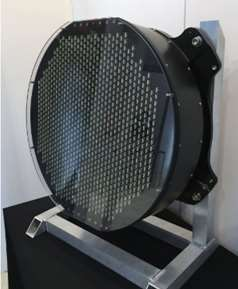
\includegraphics[width=\textwidth,height=3.5cm]{figs/aesa-antenna.png}
~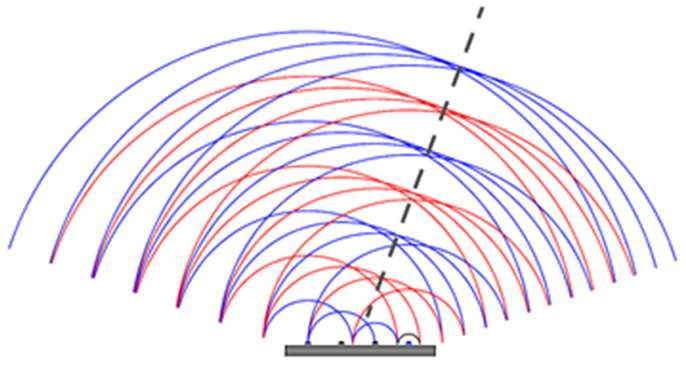
\includegraphics[width=\textwidth,height=3.5cm]{figs/aesa-beamforming.png}

Figure~\ref{fig:video-chain-spec} shows a simplified radar signal
processing chain that is used to illustrate the calculations of
interest. The input data from the antenna is processed in a number of
steps.

\begin{figure}
\hypertarget{fig:video-chain-spec}{%
\centering
\includegraphics{figs/video-chain-spec.pdf}
\caption{Overview of the video processing
chain}\label{fig:video-chain-spec}
}
\end{figure}

In this report we assume one stream per antenna element. The indata is
organized into a sequence of ``cubes'', each corresponding to a certain
integration interval. Each sample in the cube represents a particular
antenna element, pulse and range bin. The data of the cube arrives pulse
by pulse and each pulse arrives range bin by range bin. This is for all
elements in parallel. Between the Pulse Compression (PC) and Doppler
Filter Bank (DFB) steps there is a corner turn of data, i.e.~data from
all pulses must be collected before the DFB can execute.

The different steps of the chain, the antenna and the input data format
are briefly described in the following list. For a more detailed
description of the processing chain, please refer to
sections~\ref{sec:shallow}, \ref{sec:atom} respectively.

\begin{itemize}
\item
  \emph{Digital Beam Forming (DBF)}: The DBF step creates a number of
  simultaneous receiver beams, or ``listening directions'', from the
  input data. This is done by doing weighted combinations of the data
  from the different antenna elements, so that constructive interference
  is created in the desired bearings of the beams. The element samples
  in the input data set are then transformed into beams.
\item
  \emph{Pulse Compression (PC)}: The goal of the pulse compression is to
  collect all received energy from one target into a single range bin.
  The received echo of the modulated pulse is passed through a matched
  filter. Here, the matched filtering is done digitally.
\item
  \emph{Doppler Filter Bank incl.~envelope detection (DFB)}: The DFB
  gives an estimation of the target's speed relative to the radar. It
  also gives an improved signal-to-noise ratio due to a coherent
  integration of indata. The pulse bins in the data set are transformed
  into Doppler channels. The envelope detector calculates the absolute
  values of the digital samples. The data is real after this step.
\item
  \emph{Constant False Alarm Ratio (CFAR)}: The CFAR processing is
  intended to keep the number of false targets at an acceptable level
  while maintaining the best possible sensitivity. It normalizes the
  video in order to maintain a constant false alarm rate when the video
  is compared to a detection threshold. With this normalization the
  sensitivity will be adapted to the clutter situation in the area
  (around a cell under test) of interest.
\item
  \emph{Integrator (INT)} The integrator is an 8-tap unsigned integrator
  that integrates channel oriented video. Integration shall be done over
  a number of FFT batches of envelope detected video. Each Doppler
  channel, range bin and antenna element shall be integrated.
\end{itemize}

\hypertarget{sec:usage}{%
\subsection{Using This Document}\label{sec:usage}}

\textbf{PREREQUISITES:} the document assumes that the reader is familiar
with the functional programming language
\href{https://www.haskell.org/}{Haskell}, its syntax, and the usage of a
Haskell interpreter
(e.g.~\href{https://downloads.haskell.org/~ghc/latest/docs/html/users_guide/ghci.html}{\texttt{ghci}}).
Otherwise, we recommend consulting at least the introductory chapters of
one of the following books by Lipovača
(\protect\hyperlink{ref-Lipovaca11}{2011}) and Hutton
(\protect\hyperlink{ref-hutton-2016}{2016}) or other recent books in
Haskell. The reader also needs to be familiar with some basic ForSyDe
modeling concepts, such as \emph{process constructor}, \emph{process} or
\emph{signal}. We recommend going through at least the online getting
started
\href{https://forsyde.github.io/forsyde-shallow/getting_started}{tutorial
on ForSyDe-Shallow} or the one
\href{https://forsyde.github.io/forsyde-atom/assets/manual.pdf}{on
ForSyDe-Atom}, and if possible, consulting the (slightly outdated) book
chapter on ForSyDe ({\textbf{???}}).

This document has been created using literate programming. This means
that all code shown in the listings is compilable and executable. There
are two types of code listing found in this document. This style

\begin{Shaded}
\begin{Highlighting}[numbers=left,,]
\CommentTok{-- | API documentation comment}
\OtherTok{myIdFunc ::}\NormalTok{ a }\OtherTok{->}\NormalTok{ a}
\NormalTok{myIdFunc }\FunctionTok{=} \FunctionTok{id}
\end{Highlighting}
\end{Shaded}

shows \emph{source code} as it is found in the implementation files,
where the line numbers correspond to the position in the source file.
This style

\begin{verbatim}
Prelude> 1 + 1
2
\end{verbatim}

suggests \emph{interactive commands} given by the user in a terminal or
an interpreter session. The listing above shows a typical \texttt{ghci}
session, where the string after the prompter symbol
\texttt{\textgreater{}} suggests the user input (e.g.~\texttt{1\ +\ 1}).
Whenever relevant, the expected output is printed one row below
(e.g.~\texttt{2}).

The way this document is meant to be parsed efficiently is to load the
source files themselves in an interpreter and test the exported
functions gradually, while reading the document at the same time. Due to
multiple (sometimes conflicting) dependencies on external packages, for
convenience the source files are shipped as \emph{multiple}
\href{https://docs.haskellstack.org/en/stable/README/}{Stack} packages
each creating an own sandbox on the user's local machine with all
dependencies and requirements taken care of. Please refer to the
project's \texttt{README} file for instructions on how to install and
compile or run the Haskell files.

At the beginning of each chapter there is metadata guiding the reader
what tools and packages are used, like:

\begin{longtable}[]{@{}lll@{}}
\toprule
\endhead
Package & aesa-atom-0.1.0 & path:
\texttt{./aesa-atom/README.md}\tabularnewline
\bottomrule
\end{longtable}

This table tells that the package where the current chapter's code
resides is \texttt{aesa-atom}, version 0.1.0. This table might contain
information on the main dependency packages which contain important
functions, and which should be consulted while reading the code in the
current chapter. If the main package generates an executable binary or a
test suite, these are also pointed out. The third column provides
additional information such as a pointer to documentation (relative path
to the project root, or web URL), or usage suggestions.

It is recommended to read the main package's \texttt{README} file which
contains instructions on how to install, compile and test the software,
before proceeding with following a chapter. Each section of a chapter is
written within a library \emph{module}, pointed out in the beginning of
the respective section by the line:

\begin{Shaded}
\begin{Highlighting}[numbers=left,,]
\KeywordTok{module} \DataTypeTok{ForSyDe.X.Y} \KeywordTok{where}
\end{Highlighting}
\end{Shaded}

The most convenient way to test out all functions used in module
\texttt{ForSyDe.X.Y} is by loading its source file in the sandboxed
interpreter, i.e.~by running the following command from the project
root:

\begin{verbatim}
stack ghci src/ForSyDe/X/Y.lhs
\end{verbatim}

An equally convenient way is to create an own \texttt{.hs} file
somewhere under the project root, which imports and uses module
\texttt{ForSyDe.X.Y}, e.g.

\begin{Shaded}
\begin{Highlighting}[numbers=left,,]
\CommentTok{-- MyTest.hs}
\KeywordTok{import} \DataTypeTok{ForSyDe.X.Y}

\NormalTok{myData }\FunctionTok{=}\NormalTok{ [}\DecValTok{1}\NormalTok{,}\DecValTok{2}\NormalTok{,}\DecValTok{3}\NormalTok{,}\DecValTok{4}\NormalTok{,}\DecValTok{5}\NormalTok{]}\OtherTok{ ::}\NormalTok{ [}\DataTypeTok{Int}\NormalTok{]}
\NormalTok{myTest }\FunctionTok{=}\NormalTok{ functionFromForSyDeXY myData}
\end{Highlighting}
\end{Shaded}

This file can be loaded and/or compiled from within the sandbox,
e.g.~with \texttt{stack\ ghci\ MyTest.hs}.

\clearpage

\hypertarget{sec:atom}{%
\section{High-Level Model of the AESA Signal Processing Chain in
ForSyDe-Atom}\label{sec:atom}}

\begin{quote}
\emph{This section guides the reader throughout translating
``word-by-word'' the provided specifications of the AESA signal
processing chain into a concrete, functionally complete, high-level
executable model in ForSyDe-Atom. This first attempt focuses mainly on
the top-level functional behavior of the system, exerting the successive
transformations upon the input video cubes, as suggested by
Figure~\ref{fig:video-chain-spec}. We postpone the
description/derivation of more appropriate time behaviors for later
sections. Enough AESA system details are given in order to understand
the model. At the end of this section we simulate this model against a
realistic input set of complex antenna data, and test if it is sane
(i.e.~provides the expected results).}
\end{quote}

\begin{longtable}[]{@{}lll@{}}
\toprule
\endhead
Package & aesa-atom-0.1.0 & path:
\texttt{./aesa-atom/README.md}\tabularnewline
Deps & forsyde-atom-0.2.2 & url:
\texttt{https://forsyde.github.io/forsyde-atom/api/}\tabularnewline
& forsyde-atom-extensions-0.1.1 & path:
\texttt{./forsyde-atom-extensions/README.md}\tabularnewline
Bin & aesa-hl & usage: \texttt{aesa-hl\ -\/-help}\tabularnewline
\bottomrule
\end{longtable}

Historically,
\href{https://forsyde.github.io/forsyde-atom/}{ForSyDe-Atom} has been a
spin-off of
\href{https://forsyde.github.io/forsyde-shallow/}{ForSyDe-Shallow} which
has explored new modeling concepts, and had a fundamentally different
approach to how models are described and instantiated. ForSyDe-Atom
introduced the concept of \emph{language layer}, extending the idea of
process constructor, and within this setting it explored the algebra of
algorithmic skeletons, employed heavily within this report. As of today,
both ForSyDe-Shallow and ForSyDe-Atom have similar APIs and are capable
of modeling largely the same behaviors. The main syntax differences
between the two are covered in section~\ref{sec:shallow}, where the same
high-level model is written in ForSyDe-Shallow.

\hypertarget{sec:crash-atom}{%
\subsection{Crash course in ForSyDe-Atom}\label{sec:crash-atom}}

Before proceeding with the modeling of the AESA processing chain, let us
consolidate the main ForSyDe concepts which will be used throughout this
report: \emph{layer}, \emph{process constructor} and \emph{skeleton}. If
you are not familiar with ForSyDe nomenclature and general modeling
principles, we recommend consulting the documentation pointed out in
section~\ref{sec:intro} first.

As seen in section~\ref{sec:video-chain-spec}, most of the AESA
application consists of typical DSP algorithms such as matrix
multiplications, FFT, moving averages, etc. which lend themselves to
\emph{streaming parallel} implementations. Hence we need to
unambiguously capture the two distinct aspects of the AESA chain
components:

\begin{itemize}
\item
  \emph{streaming behavior} is expressed in ForSyDe through processes
  which operate on signals encoding a temporal partitioning of data.
  Processes are instantiated exclusively using \emph{process
  constructors} which can be regarded as templates inferring the
  semantics of computation, synchronization and concurrency as dictated
  by a certain model of computation (MoC) (Sander and Jantsch
  (\protect\hyperlink{ref-sander-2004}{2004}),Lee and Seshia
  (\protect\hyperlink{ref-leeseshia-15}{2016})).
\item
  \emph{parallelism} is expressed through parallel patterns which
  operate on structured types (e.g.~vectors) encoding a spatial
  partitioning of data. These patterns are instantiated as skeletons,
  which are templates inferring the semantics of distribution, parallel
  computation and interaction between elements, as defined by the
  algebra of catamorphisms (Fischer, Gorlatch, and Bischof
  \protect\hyperlink{ref-Fischer-2003}{2003}).
\end{itemize}

\begin{figure}
\hypertarget{fig:atom-layers}{%
\centering
\includegraphics{figs/layers.pdf}
\caption{Depiction of layer usage: (left) skeleton networks of
processes; (right) processes of skeleton
functions}\label{fig:atom-layers}
}
\end{figure}

In order to capture these two\footnote{and other aspects, not covered in
  this report} interacting aspects in unison as a complete system, we
describe them in terms of two distinct, orthogonal \emph{layers} within
the ForSyDe-Atom framework. A language layer is a (very small) domain
specific language (DSL) heavily rooted in the functional programming
paradigm, which is able to describe one aspect of a cyber-physical
system (CPS). Layers interact with one another by virtue of the
abstraction principle inherent to a functional programming language
(Backus \protect\hyperlink{ref-backus-1978}{1978}): each layer defines
at least one higher order function that is able to take a function
(i.e.~abstraction) from another layer as an argument and to lift it
within its own domain. To nepicture the interaction between layers,
consider Figure~\ref{fig:video-chain-spec} where, although we use the
same \texttt{farm} vector skeleton and \texttt{comb} synchronous (SY)
process constructor, the two different compositions describe two
different (albeit semantically equivalent) systems: the first one is
instantiating a farm network of SY processes operating on a vector of
signals in parallel; whereas the second one is instantiating a single SY
process operating on o signal where each event is carrying a vector of
values.

\hypertarget{sec:cube-atom-operation}{%
\subsection{A High-Level Model}\label{sec:cube-atom-operation}}

This section presents a high-level behavioral model of the AESA signal
processing chain presented in section~\ref{sec:video-chain-spec}. This
model follows intuitive and didactic way to tackle the challenge of
translating the \emph{textual} specifications into an \emph{executable}
ForSyDe specification and is not, in any circumstance, the only way to
model the application. As of section~\ref{sec:crash-atom} we represent
each stage in the AESA chain as a \emph{process} acting upon (complete)
\emph{cubes} of data, i.e.~as processes of skeleton functions. At this
phase in the system design we do not care \emph{how} the cubes are being
formed or how the data is being carried around, bur rather on
\emph{what} transformations are applied on the data cubes during each
subsequent stage of the AESA pipeline. The purpose of the model is to
provide a executable \emph{reference} for the AESA system functionality,
that can later be derived to more efficient descriptions.

The code for this section is written in the following module, see
section~\ref{sec:usage} on how to use it:

\begin{Shaded}
\begin{Highlighting}[numbers=left,,firstnumber=18,]
\OtherTok{\{-# LANGUAGE PackageImports #-\}} \CommentTok{-- allows explicit import of modules from custom}
                                \CommentTok{-- libraries instead of standard ones. Will be taken}
                                \CommentTok{-- out once the extensions are merged upstream.}
\KeywordTok{module} \DataTypeTok{ForSyDe.AESA.CubesAtom} \KeywordTok{where}
\end{Highlighting}
\end{Shaded}

As the AESA application uses complex numbers, we use Haskell's
\href{http://hackage.haskell.org/package/base/docs/Data-Complex.html}{\texttt{Complex}}
type.

\begin{Shaded}
\begin{Highlighting}[numbers=left,,firstnumber=26,]
\KeywordTok{import} \DataTypeTok{Data.Complex}
\end{Highlighting}
\end{Shaded}

The only timed behavior exerted by the model in this section is the
causal, i.e.~ordered, passing of cubes from one stage to another. In
order to enable a simple, abstract, and thus analyzable ``pipeline''
behavior this passing can be described according to the \emph{perfect
synchrony hypothesis}, which assumes the processing of each event (cube)
takes an infinetly small amount of time and it is ready before the next
sinchronization point. This in turn implies that all events in a system
are synchronized, enabling the description of fully deterministic
behaviors over infinite streams of events. These precise execution
semantics are captured by the \emph{synchronous reactive (SY) model of
computation (MoC)} (Lee and Seshia
(\protect\hyperlink{ref-leeseshia-15}{2016}),Benveniste et al.
(\protect\hyperlink{ref-Benveniste03}{2003})), hence we import the
\href{https://forsyde.github.io/forsyde-atom/api/ForSyDe-Atom-MoC-SY.html}{\texttt{SY}}
library from the
\emph{\href{https://forsyde.github.io/forsyde-atom/api/ForSyDe-Atom-MoC.html}{MoC}
layer} of ForSyDe-Atom, see (Ungureanu and Sander
\protect\hyperlink{ref-ungureanu17}{2017}), using an appropriate alias.

\begin{Shaded}
\begin{Highlighting}[numbers=left,,firstnumber=42,]
\KeywordTok{import}\NormalTok{ "forsyde-atom-extensions" }\DataTypeTok{ForSyDe.Atom.MoC.SY}  \KeywordTok{as} \DataTypeTok{SY}
\end{Highlighting}
\end{Shaded}

For describing parallel operations on data we use algorithmic skeletons
(Fischer, Gorlatch, and Bischof
(\protect\hyperlink{ref-Fischer-2003}{2003}),Skillicorn
(\protect\hyperlink{ref-skillicorn05}{2005})), formulated on
ForSyDe-Atom's in-house
\href{http://hackage.haskell.org/package/forsyde-shallow/docs/ForSyDe-Shallow-Core-Vector.html}{\texttt{Vector}}
data type, which is a shallow, lazy-evaluated implementation of
unbounded arrays, ideal for early design validation. Although dependent,
bounded, and even boxed (i.e.~memory-mapped) alternatives exist, such as
\href{http://hackage.haskell.org/package/parameterized-data/docs/Data-Param-FSVec.html}{\texttt{FSVec}}
or REPA \href{http://hackage.haskell.org/package/repa}{\texttt{Array}}s,
for the scope of this project the functional validation and (by-hand)
requirement analysis on the properties of skeletons will suffice. We
also import the \texttt{Matrix} and \texttt{Cube} utility libraries
which contain type synonyms for nested \texttt{Vector}s along with their
derived skeletons, as well a \texttt{DSP} which contain commonly used
DSP blocks defined in terms of vector skeletons.

\begin{Shaded}
\begin{Highlighting}[numbers=left,,firstnumber=58,]
\KeywordTok{import}\NormalTok{ "forsyde-atom-extensions" }\DataTypeTok{ForSyDe.Atom.Skeleton.Vector}        \KeywordTok{as} \DataTypeTok{V}
\KeywordTok{import}\NormalTok{ "forsyde-atom-extensions" }\DataTypeTok{ForSyDe.Atom.Skeleton.Vector.Matrix} \KeywordTok{as} \DataTypeTok{M}
\KeywordTok{import}\NormalTok{ "forsyde-atom-extensions" }\DataTypeTok{ForSyDe.Atom.Skeleton.Vector.Cube}   \KeywordTok{as} \DataTypeTok{C}
\KeywordTok{import}\NormalTok{ "forsyde-atom-extensions" }\DataTypeTok{ForSyDe.Atom.Skeleton.Vector.DSP}
\end{Highlighting}
\end{Shaded}

Finally, we import the local project module defining different
coefficients for the AESA algorithms, presented in detail in
section~\ref{sec:coefs-atom}.

\begin{Shaded}
\begin{Highlighting}[numbers=left,,firstnumber=66,]
\KeywordTok{import} \DataTypeTok{ForSyDe.AESA.Coefs}
\end{Highlighting}
\end{Shaded}

\hypertarget{sec:cube-aliases-shallow}{%
\subsubsection{Type Aliases and
Constants}\label{sec:cube-aliases-shallow}}

The system parameters are integer constants defining the size of the
application. For a simple test scenario provided by Saab AB, we have
bundled these parameters in the following module, and we shall use their
variable names throughout the whole report:

\begin{Shaded}
\begin{Highlighting}[numbers=left,,firstnumber=74,]
\KeywordTok{import} \DataTypeTok{ForSyDe.AESA.Params}
\end{Highlighting}
\end{Shaded}

For ease of documentation we will be using type synonyms (aliases) for
all types and structures throughout this design:

\begin{itemize}
\item
  \texttt{Antenna} denotes a vector container for the antenna elements.
  Its length is equal to the number of antennas in the radar \(N_A\).
\item
  After Digital Beamforming (DBF), the antenna elements are transformed
  into \(N_B\) beams, thus we associate the \texttt{Beam} alias for the
  vector container wrapping those beams.
\item
  \texttt{Range} is a vector container for range bins. All antennas have
  the same number of range bins \(N_b\), rendering each
  \(\text{Antenna} \times \text{Range}\) a perfect matrix of samples for
  every pulse.
\item
  \texttt{Window} stands for a Doppler window of \(N_{FFT}\) pulses.
\end{itemize}

\begin{Shaded}
\begin{Highlighting}[numbers=left,,firstnumber=92,]
\KeywordTok{type} \DataTypeTok{Antenna}     \FunctionTok{=} \DataTypeTok{Vector} \CommentTok{-- length: nA}
\KeywordTok{type} \DataTypeTok{Beam}        \FunctionTok{=} \DataTypeTok{Vector} \CommentTok{-- length: nB}
\KeywordTok{type} \DataTypeTok{Range}       \FunctionTok{=} \DataTypeTok{Vector} \CommentTok{-- length: nb}
\KeywordTok{type} \DataTypeTok{Window}      \FunctionTok{=} \DataTypeTok{Vector} \CommentTok{-- length: nFFT}
\end{Highlighting}
\end{Shaded}

Finally we provide two aliases for the basic Haskell data types used in
the system, to stay consistent with the application specification.

\begin{Shaded}
\begin{Highlighting}[numbers=left,,firstnumber=100,]
\KeywordTok{type} \DataTypeTok{CpxData}  \FunctionTok{=} \DataTypeTok{Complex} \DataTypeTok{Float}
\KeywordTok{type} \DataTypeTok{RealData} \FunctionTok{=} \DataTypeTok{Float}
\end{Highlighting}
\end{Shaded}

\hypertarget{video-processing-pipeline-stages}{%
\subsubsection{Video Processing Pipeline
Stages}\label{video-processing-pipeline-stages}}

In this section we follow each stage described in
section~\ref{sec:video-chain-spec}, and model them as a processes
operating on cubes (three-dimensional vectors) of antenna samples.

\hypertarget{sec:cube-dbf-atom}{%
\paragraph{Digital Beamforming (DFB)}\label{sec:cube-dbf-atom}}

The DBF receives complex in data, from \(N_A\) antenna elements and
forms \(N_B\) simultaneous receiver beams, or ``listening directions'',
by summing individually phase-shifted in data signals from all elements.
Considering the indata video cube, the transformation applied by DBF,
could be depicted as in Figure~\ref{fig:cube-dbf-cube}.

\begin{figure}
\hypertarget{fig:cube-dbf-cube}{%
\centering
\includegraphics{figs/dbf-cube.pdf}
\caption{DBF on video structure}\label{fig:cube-dbf-cube}
}
\end{figure}

Considering the application specification in
section~\ref{sec:video-chain-spec} on the input data, namely \emph{``for
each antenna the data arrives \emph{pulse by pulse}, and each pulse
arrives \emph{range bin by range bin}''}, we can assume that the video
is received as \texttt{Antenna\ (Window\ (Range\ a))} cubes, meaning
that the inner vectors are the range bins. However,
Figure~\ref{fig:cube-dbf-cube} shows that the beamforming function is
applied in the antenna direction, so we need to transpose the cube in
such a way that \texttt{Antenna} becomes the inner vector,
i.e.~\texttt{Window\ (Range\ (Antenna\ a))}. We thus describe the DBF
stage as a combinational SY process \texttt{comb} acting upon signals of
\texttt{Cube}s, namely mapping the beamforming function \(f_{DBF}\) on
each column of each \emph{pulse matrix} (see
Figure~\ref{fig:cube-dbf-cube}).

\begin{figure}
\hypertarget{fig:cube-dbf-proc-shallow}{%
\centering
\includegraphics{figs/dbf-proc-atom.pdf}
\caption{DBF stage process}\label{fig:cube-dbf-proc-shallow}
}
\end{figure}

\begin{Shaded}
\begin{Highlighting}[numbers=left,,firstnumber=130,]
\OtherTok{dbf ::} \DataTypeTok{Signal}\NormalTok{ (}\DataTypeTok{Antenna}\NormalTok{ (}\DataTypeTok{Window}\NormalTok{ (}\DataTypeTok{Range} \DataTypeTok{CpxData}\NormalTok{)))}
    \OtherTok{->} \DataTypeTok{Signal}\NormalTok{ (}\DataTypeTok{Window}\NormalTok{  (}\DataTypeTok{Range}\NormalTok{  (}\DataTypeTok{Beam}  \DataTypeTok{CpxData}\NormalTok{)))}
\NormalTok{dbf }\FunctionTok{=}\NormalTok{ SY.comb11 (M.farm11 fDBF }\FunctionTok{.}\NormalTok{ C.transpose)}
\end{Highlighting}
\end{Shaded}

The beamforming function is specified like in eq.~\ref{eq:dbf}, where
\(e_k ,\ \forall k \in [1,N_A]\) denotes the samples from antenna
elements, and respectively \(b_i,\ \forall i \in [1,N_B]\) are samples
for each beam. This is in fact a of matrix-vector multiplication, thus
we implement eq.~\ref{eq:dbf} at the highest level of abstraction simply
as matrix/vector operations like in eq.~\ref{eq:dbf-mat}.

\begin{equation} b_i(n) = \sum_{k=1}^{N_A} e_k(n) \cdot \alpha_{ki}\qquad\forall i \in [1,N_B] \label{eq:dbf}\end{equation}

\begin{Shaded}
\begin{Highlighting}[numbers=left,,firstnumber=142,]
\OtherTok{fDBF ::} \DataTypeTok{Antenna} \DataTypeTok{CpxData} \CommentTok{-- ^ input antenna elements}
     \OtherTok{->} \DataTypeTok{Beam}    \DataTypeTok{CpxData} \CommentTok{-- ^ output beams}
\NormalTok{fDBF antennaEl }\FunctionTok{=}\NormalTok{ beam}
  \KeywordTok{where}
\NormalTok{    beam       }\FunctionTok{=}\NormalTok{ V.reduce (V.farm21 (}\FunctionTok{+}\NormalTok{)) beamMatrix}
\NormalTok{    beamMatrix }\FunctionTok{=}\NormalTok{ M.farm21 (\textbackslash{}c }\OtherTok{->}\NormalTok{ (}\FunctionTok{*}\NormalTok{c)) beamConsts elMatrix}
\NormalTok{    elMatrix   }\FunctionTok{=}\NormalTok{ V.farm11 V.fanout antennaEl}
\NormalTok{    beamConsts }\FunctionTok{=}\NormalTok{ mkBeamConsts dElements waveLength nA}\OtherTok{ nB ::} \DataTypeTok{Matrix} \DataTypeTok{CpxData}
\end{Highlighting}
\end{Shaded}

\begin{longtable}[]{@{}lll@{}}
\toprule
Function & Original module & Package\tabularnewline
\midrule
\endhead
\texttt{farm11}, \texttt{reduce}, \texttt{length} &
\href{https://forsyde.github.io/forsyde-atom/api/ForSyDe-Atom-Skeleton-Vector.html}{\texttt{ForSyDe.Atom.Skeleton.Vector}}
& forsyde-atom\tabularnewline
\texttt{farm11}, \texttt{farm21} &
\texttt{ForSyDe.Atom.Skeleton.Vector.Matrix} &
forsyde-atom-extensions\tabularnewline
\texttt{transpose} & \texttt{ForSyDe.Atom.Skeleton.Vector.Cube} &
forsyde-atom-extensions\tabularnewline
\texttt{comb11} &
\href{https://forsyde.github.io/forsyde-atom/api/ForSyDe-Atom-MoC-SY.html}{\texttt{ForSyDe.Atom.MoC.SY}}
& forsyde-atom\tabularnewline
\texttt{mkBeamConsts} & \texttt{ForSyDe.AESA.Coefs} &
aesa-atom\tabularnewline
\texttt{dElements}, \texttt{waveLenth}, \texttt{nA}, \texttt{nB} &
\texttt{ForSyDe.AESA.Params} & aesa-atom\tabularnewline
\bottomrule
\end{longtable}

\begin{equation} \begin{gathered}
   \stackrel{\mbox{elMatrix}}{
   \begin{bmatrix}
    e_{1} & e_{1} & \dots  \\
    e_{2} & e_{2} & \dots  \\
    \vdots& \vdots& \ddots \\
    e_{N_A} & e_{N_A} & \dots
   \end{bmatrix}}
   \times
   \stackrel{\mbox{beamConsts}}{
   \begin{bmatrix}
    \alpha_{11} & \alpha_{12} & \dots  & \alpha_{1N_B} \\
    \alpha_{21} & \alpha_{22} & \dots  & \alpha_{2N_B} \\
    \vdots      & \vdots      & \ddots & \vdots\\
    \alpha_{N_A1} & \alpha_{N_A2} & \dots  & \alpha_{N_AN_B} 
   \end{bmatrix}}
   \Rightarrow\\\Rightarrow
   \stackrel{\mbox{beamMatrix}}{
   \left.\begin{bmatrix}
    e_1\alpha_{11} & e_1\alpha_{12} & \dots  & e_1\alpha_{1N_B} \\
    e_2\alpha_{21} & e_2\alpha_{22} & \dots  & e_2\alpha_{2N_B} \\
    \vdots & \vdots & \ddots & \vdots\\
    e_{N_A}\alpha_{N_A1} & e_{N_A}\alpha_{N_A2} & \dots  & e_{N_A}\alpha_{N_AN_B} 
   \end{bmatrix}\right\}}
   \sum_\mathit{rows}=
   \stackrel{\mbox{beam}}{
   \begin{bmatrix}
    b_1 & b_2 & \dots  & b_n 
   \end{bmatrix}}
   \end{gathered}
\label{eq:dbf-mat}\end{equation}

\hypertarget{sec:cube-pc-atom}{%
\paragraph{Pulse Compression (PC)}\label{sec:cube-pc-atom}}

In this stage the received echo of the modulated pulse, i.e.~the
information contained by the range bins, is passed through a matched
filter for decoding their modulation. This essentially applies a sliding
window, or a moving average on the range bin samples. Considering the
video cube, the PC transformation is applied in the direction shown in
Figure~\ref{fig:cube-pc-cube}, i.e.~on vectors formed from the range of
every pulse.

\begin{figure}
\hypertarget{fig:cube-pc-cube}{%
\centering
\includegraphics{figs/pc-cube.pdf}
\caption{PC: direction of application on video structure (left); process
(right)}\label{fig:cube-pc-cube}
}
\end{figure}

The PC process is mapping the \(f_{PC}\) on each row of the pulse
matrices in a cube, however the previous stage has arranged the cube to
be aligned beam-wise. This is why we need to re-arrange the data so that
the innermost vectors are \texttt{Range}s instead, and we do this by
simply \texttt{transpose}-ing the inner \texttt{Range} \(\times\)
\texttt{Beam} matrices into \texttt{Beam} \(\times\) \texttt{Range}
ones.

\begin{Shaded}
\begin{Highlighting}[numbers=left,,firstnumber=208,]
\OtherTok{pc ::} \DataTypeTok{Signal}\NormalTok{ (}\DataTypeTok{Window}\NormalTok{ (}\DataTypeTok{Range}\NormalTok{ (}\DataTypeTok{Beam}  \DataTypeTok{CpxData}\NormalTok{))) }
   \OtherTok{->} \DataTypeTok{Signal}\NormalTok{ (}\DataTypeTok{Window}\NormalTok{ (}\DataTypeTok{Beam}\NormalTok{  (}\DataTypeTok{Range} \DataTypeTok{CpxData}\NormalTok{)))}
\NormalTok{pc }\FunctionTok{=}\NormalTok{ SY.comb11 (V.farm11 (V.farm11 fPC }\FunctionTok{.}\NormalTok{ M.transpose))}
\CommentTok{--             ^ == (M.farm11 fPC . V.farm11 M.transpose)}
\end{Highlighting}
\end{Shaded}

Here the function \(f_{PC}\) applies the \texttt{fir} skeleton on these
vectors (which computes a moving average if considering vectors). The
\texttt{fir} skeleton is a utility formulated in terms of primitive
skeletons (i.e.~\texttt{farm} and \texttt{reduce}) on numbers,
i.e.~lifting arithmetic functions. We will study this skeleton later in
this report and for now we take it ``for granted'', as conveniently
provided by the \texttt{DSP} utility library. For this application we
also use a relatively small average window (5 taps).

\begin{Shaded}
\begin{Highlighting}[numbers=left,,firstnumber=220,]
\OtherTok{fPC ::} \DataTypeTok{Range} \DataTypeTok{CpxData} \CommentTok{-- ^ input range bin     }
    \OtherTok{->} \DataTypeTok{Range} \DataTypeTok{CpxData} \CommentTok{-- ^ output pulse-compressed bin}
\NormalTok{fPC }\FunctionTok{=}\NormalTok{ fir (mkPcCoefs }\DecValTok{5}\NormalTok{)}
\end{Highlighting}
\end{Shaded}

\begin{longtable}[]{@{}lll@{}}
\toprule
\begin{minipage}[b]{0.24\columnwidth}\raggedright
Function\strut
\end{minipage} & \begin{minipage}[b]{0.41\columnwidth}\raggedright
Original module\strut
\end{minipage} & \begin{minipage}[b]{0.26\columnwidth}\raggedright
Package\strut
\end{minipage}\tabularnewline
\midrule
\endhead
\begin{minipage}[t]{0.24\columnwidth}\raggedright
\texttt{comb11}\strut
\end{minipage} & \begin{minipage}[t]{0.41\columnwidth}\raggedright
\href{https://forsyde.github.io/forsyde-atom/api/ForSyDe-Atom-MoC-SY.html}{\texttt{ForSyDe.Atom.MoC.SY}}\strut
\end{minipage} & \begin{minipage}[t]{0.26\columnwidth}\raggedright
forsyde-atom\strut
\end{minipage}\tabularnewline
\begin{minipage}[t]{0.24\columnwidth}\raggedright
\texttt{farm11}\strut
\end{minipage} & \begin{minipage}[t]{0.41\columnwidth}\raggedright
\href{https://forsyde.github.io/forsyde-atom/api/ForSyDe-Atom-Skeleton-Vector.html}{\texttt{ForSyDe.Atom.Skeleton.Vector}}\strut
\end{minipage} & \begin{minipage}[t]{0.26\columnwidth}\raggedright
forsyde-atom\strut
\end{minipage}\tabularnewline
\begin{minipage}[t]{0.24\columnwidth}\raggedright
\texttt{farm11}, \texttt{transpose}\strut
\end{minipage} & \begin{minipage}[t]{0.41\columnwidth}\raggedright
\texttt{ForSyDe.Atom.Skeleton.Vector.Matrix}\strut
\end{minipage} & \begin{minipage}[t]{0.26\columnwidth}\raggedright
forsyde-atom-extensions\strut
\end{minipage}\tabularnewline
\begin{minipage}[t]{0.24\columnwidth}\raggedright
\texttt{fir}\strut
\end{minipage} & \begin{minipage}[t]{0.41\columnwidth}\raggedright
\texttt{ForSyDe.Atom.Skeleton.Vector.DSP}\strut
\end{minipage} & \begin{minipage}[t]{0.26\columnwidth}\raggedright
forsyde-atom-extensions\strut
\end{minipage}\tabularnewline
\begin{minipage}[t]{0.24\columnwidth}\raggedright
\texttt{mkPcCoefs}\strut
\end{minipage} & \begin{minipage}[t]{0.41\columnwidth}\raggedright
\texttt{ForSyDe.AESA.Coefs}\strut
\end{minipage} & \begin{minipage}[t]{0.26\columnwidth}\raggedright
aesa-atom\strut
\end{minipage}\tabularnewline
\bottomrule
\end{longtable}

\hypertarget{sec:cube-ct-atom}{%
\paragraph{Corner Turn (CT) with 50\% overlapping
data}\label{sec:cube-ct-atom}}

During the CT a rearrangement of data must be performed between
functions that process data in ``different'' directions, e.g.~range and
pulse, in order to be able to calculate the Doppler channels further in
the processing pipeline. The process of corner turning becomes highly
relevant when detailed time behavior of the application is being derived
or inferred, since it demands well-planned design decisions to make full
use of the underlying architecture. At the level of abstraction on which
we work right now though, it is merely a matrix \texttt{transpose}
operation, and it can very well be posponed until the beginning of the
next stage. However, a much more interesting operation is depicted in
Figure~\ref{fig:cube-ct-cube}: in order to maximize the efficiency of
the AESA processing the datapath is split into two concurrent processing
channels with 50\% overlapped data.

\begin{figure}
\hypertarget{fig:cube-ct-cube}{%
\centering
\includegraphics{figs/ct-cube.pdf}
\caption{Concurrent processing on 50\% overlapped
data}\label{fig:cube-ct-cube}
}
\end{figure}

Implmeneting such a behavior requires a bit of ``ForSyDe thinking''. At
a first glance, the problem seems easily solved considering only the
cube structures: just ``ignore'' half of the first cube of the right
channel, while the left channel replicates the input. However, there are
some timing issues with this setup: from the left channel's perspective,
the right channel is in fact ``peaking into the future'', which is an
abnormal behavior. Without going too much into details, you need to
understand that \emph{any type of signal ``cleaning'', like dropping or
filtering out events, can cause serious causality issues in a generic
process network, and thus it is \textbf{illegal} in ForSyDe system
modeling}. On the other hand we could \emph{delay} the left channel in a
determinstic manner by assuming a well-defined \emph{initial state}
(e.g.~all zeroes) while it waits for the right channel to consume and
process its first half of data. This defines the history of a system
where all components start from \emph{time zero} and eliminates any
source of ``clairvoyant''/ambiguous behavior.

To keep things simple, we stay within the same time domain, keeping the
perfect synchrony assumption, and instantiating the left channel
building mechanism as a simple Mealy finite state machine. This machine
splits an input cube into two halves, stores one half and merges the
other half with the previously stored state to create the left channel
stream of cubes.

\begin{figure}
\hypertarget{fig:cube-ct-proc-atom}{%
\centering
\includegraphics{figs/ct-proc-atom.pdf}
\caption{Left channel data builder process}\label{fig:cube-ct-proc-atom}
}
\end{figure}

\begin{Shaded}
\begin{Highlighting}[numbers=left,,firstnumber=270,]
\OtherTok{overlap ::} \DataTypeTok{Signal}\NormalTok{ (}\DataTypeTok{Window}\NormalTok{ (}\DataTypeTok{Beam}\NormalTok{ (}\DataTypeTok{Range} \DataTypeTok{CpxData}\NormalTok{)))}
        \OtherTok{->} \DataTypeTok{Signal}\NormalTok{ (}\DataTypeTok{Window}\NormalTok{ (}\DataTypeTok{Beam}\NormalTok{ (}\DataTypeTok{Range} \DataTypeTok{CpxData}\NormalTok{)))}
\NormalTok{overlap }\FunctionTok{=}\NormalTok{ SY.mealy11 nextState outDecode initState}
  \KeywordTok{where}
\NormalTok{    nextState _ cube }\FunctionTok{=}\NormalTok{ V.drop (nFFT }\OtherTok{`div`} \DecValTok{2}\NormalTok{) cube}
\NormalTok{    outDecode s cube }\FunctionTok{=}\NormalTok{ s }\FunctionTok{<++>}\NormalTok{ V.take (nFFT }\OtherTok{`div`} \DecValTok{2}\NormalTok{) cube}
\NormalTok{    initState        }\FunctionTok{=}\NormalTok{ (V.fanoutn (nFFT }\OtherTok{`div`} \DecValTok{2}\NormalTok{) }\FunctionTok{.}\NormalTok{ V.fanoutn nB }\FunctionTok{.}\NormalTok{ V.fanoutn nb) }\DecValTok{0}
\end{Highlighting}
\end{Shaded}

\begin{longtable}[]{@{}lll@{}}
\toprule
Function & Original module & Package\tabularnewline
\midrule
\endhead
\texttt{mealy11} &
\href{https://forsyde.github.io/forsyde-atom/api/ForSyDe-Atom-MoC-SY.html}{\texttt{ForSyDe.Atom.MoC.SY}}
& forsyde-atom\tabularnewline
\texttt{drop}, \texttt{take}, \texttt{fanoutn},
\texttt{(\textless{}++\textgreater{})} &
\href{https://forsyde.github.io/forsyde-atom/api/ForSyDe-Atom-Skeleton-Vector.html}{\texttt{ForSyDe.Atom.Skeleton.Vector}}
& forsyde-atom\tabularnewline
\texttt{nFFT}, \texttt{nA}, \texttt{nB} & \texttt{ForSyDe.AESA.Params} &
aesa-atom\tabularnewline
\bottomrule
\end{longtable}

\textbf{OBS!} Perhaps considering all zeroes for the initial state might
not be the best design decision, since that is in fact ``junk data''
which is propagated throughout the system and which alters the expected
behavior. A much safer (and semantically correct) approach would be to
model the initial state using \emph{absent events} instead of arbitrary
data. However this demands the introduction of a new layer and some
quite advanced modeling concepts which are out of the scope of this
report\footnote{For more information on absent semantics, check out
  Chapter 3 of (Lee and Seshia
  \protect\hyperlink{ref-leeseshia-15}{2016})}. For the sake of
simplicity we now consider that the initial state is half a cube of
zeroes and that there are no absent events in the system. As earlier
mentioned, it is \emph{illegal} to assume any type of signal cleaning
during system modeling, however this law does not apply to the
\emph{observer} (i.e.~the testbench), who is free to take into
consideration whichever parts of the signals it deems necessary. We will
abuse this knowledge in order to show a realistic output behavior of the
AESA signal processing system: as ``observers'', we will ignore the
effects of the initial state propagation from the output signal and
instead plot only the useful data.

\hypertarget{sec:cube-dfb-atom}{%
\paragraph{Doppler Filter Bank (DFB)}\label{sec:cube-dfb-atom}}

During the Doppler filter bank, every window of samples, associated with
each range bin is transformed into a Doppler channel and the complex
samples are converted to real numbers by calculating their envelope. The
DFB transformation is applied over a window of \(N_{FFT}\) samples, thus
we need to re-arrange the data cubes again as suggested in
Figure~\ref{fig:cube-dfb-samp}.

The \texttt{dfb} process applies the the following chain of functions on
each window of complex samples, in three consecutive steps:

\begin{itemize}
\item
  scale the window samples with a set of coefficients to decrease the
  Doppler side lobes from each FFT output and thereby to increase the
  clutter rejection.
\item
  apply an \(N_{FFT}\)-point 2-radix decimation in frequency Fast
  Fourier Transform (FFT) algorithm.
\item
  compute the envelope of each complex sample when phase information is
  no longer of interest. The envelope is obtained by calculating the
  absolute value of the complex number, converting it into a real
  number.
\end{itemize}

\begin{longtable}[]{@{}lll@{}}
\toprule
Function & Original module & Package\tabularnewline
\midrule
\endhead
\texttt{farm11},\texttt{farm21} &
\href{https://forsyde.github.io/forsyde-atom/api/ForSyDe-Atom-Skeleton-Vector.html}{\texttt{ForSyDe.Atom.Skeleton.Vector}}
& forsyde-atom\tabularnewline
\texttt{fft} & \texttt{ForSyDe.Atom.Skeleton.Vector.DSP} &
forsyde-atom-extensions\tabularnewline
\texttt{mkWeightCoefs} & \texttt{ForSyDe.AESA.Coefs} &
aesa-atom\tabularnewline
\texttt{nS}, \texttt{nFFT} & \texttt{ForSyDe.AESA.Params} &
aesa-atom\tabularnewline
\bottomrule
\end{longtable}

\begin{figure}
\hypertarget{fig:cube-dfb-cube}{%
\centering
\includegraphics{figs/dfb-cube.pdf}
\caption{Doppler Filter Bank on video
structure}\label{fig:cube-dfb-cube}
}
\end{figure}

\begin{figure}
\hypertarget{fig:cube-dfb-proc-atom}{%
\centering
\includegraphics{figs/dfb-proc-atom.pdf}
\caption{DFB process}\label{fig:cube-dfb-proc-atom}
}
\end{figure}

\begin{Shaded}
\begin{Highlighting}[numbers=left,,firstnumber=333,]
\OtherTok{dfb ::} \DataTypeTok{Signal}\NormalTok{ (}\DataTypeTok{Window}\NormalTok{ (}\DataTypeTok{Beam}\NormalTok{  (}\DataTypeTok{Range}  \DataTypeTok{CpxData}\NormalTok{ )))}
    \OtherTok{->} \DataTypeTok{Signal}\NormalTok{ (}\DataTypeTok{Beam}\NormalTok{   (}\DataTypeTok{Range}\NormalTok{ (}\DataTypeTok{Window} \DataTypeTok{RealData}\NormalTok{)))}
\NormalTok{dfb }\FunctionTok{=}\NormalTok{ SY.comb11 (M.farm11 fDFB }\FunctionTok{.}\NormalTok{ C.transpose)}

\OtherTok{fDFB ::} \DataTypeTok{Window} \DataTypeTok{CpxData} \OtherTok{->} \DataTypeTok{Window} \DataTypeTok{RealData}
\NormalTok{fDFB }\FunctionTok{=}\NormalTok{ V.farm11 envelope }\FunctionTok{.}\NormalTok{ fft nS }\FunctionTok{.}\NormalTok{ weight}
  \KeywordTok{where}
\NormalTok{    weight     }\FunctionTok{=}\NormalTok{ V.farm21 (}\FunctionTok{*}\NormalTok{) (mkWeightCoefs nFFT)}
\NormalTok{    envelope a }\FunctionTok{=} \KeywordTok{let}\NormalTok{ (i, q) }\FunctionTok{=}\NormalTok{ (realPart a, imagPart a)}
                 \KeywordTok{in} \FunctionTok{sqrt}\NormalTok{ (i }\FunctionTok{*}\NormalTok{ i }\FunctionTok{+}\NormalTok{ q }\FunctionTok{*}\NormalTok{ q)}
\end{Highlighting}
\end{Shaded}

\hypertarget{sec:cube-cfar-atom}{%
\paragraph{Constant False Alarm Ratio (CFAR)}\label{sec:cube-cfar-atom}}

The CFAR normalizes the data within the video cubes in order to maintain
a constant false alarm rate with respect to a detection threshold. This
is done in order to keep the number of false targets at an acceptable
level by adapting the normalization to the clutter situation in the area
(around a cell under test) of interest. The described process can be
depicted as in Figure~\ref{fig:cube-cfar-cube} which suggests the
\href{https://en.wikipedia.org/wiki/Stencil_code}{stencil} data
accessing pattern within the video cubes.

\begin{figure}
\hypertarget{fig:cube-cfar-cube}{%
\centering
\includegraphics{figs/cfar-cube.pdf}
\caption{Constant False Alarm Ratio on cubes of complex
samples}\label{fig:cube-cfar-cube}
}
\end{figure}

\begin{Shaded}
\begin{Highlighting}[numbers=left,,firstnumber=356,]
\OtherTok{cfar ::} \DataTypeTok{Signal}\NormalTok{ (}\DataTypeTok{Beam}\NormalTok{ (}\DataTypeTok{Range}\NormalTok{ (}\DataTypeTok{Window} \DataTypeTok{RealData}\NormalTok{)))}
     \OtherTok{->} \DataTypeTok{Signal}\NormalTok{ (}\DataTypeTok{Beam}\NormalTok{ (}\DataTypeTok{Range}\NormalTok{ (}\DataTypeTok{Window} \DataTypeTok{RealData}\NormalTok{)))}
\NormalTok{cfar }\FunctionTok{=}\NormalTok{ SY.comb11 (V.farm11 fCFAR)}
\end{Highlighting}
\end{Shaded}

\begin{figure}
\hypertarget{fig:cube-cfar-proc-atom}{%
\centering
\includegraphics{figs/cfar-proc-atom.pdf}
\caption{CFAR process}\label{fig:cube-cfar-proc-atom}
}
\end{figure}

The \texttt{cfar} process applies the \(f_{CFAR}\) function on every
\(N_b\times N_{FFT}\) matrix corresponding to each beam. The
\(f_{CFAR}\) function normalizes each Doppler window, after which the
sensitivity will be adapted to the clutter situation in current area, as
seen in Figure~\ref{fig:cube-cfar-signal}. The blue line indicates the
mean value of maximum of the left and right reference bins, which means
that for each Doppler sample, a swipe of neighbouring bins is necessary,
as suggested by Figure~\ref{fig:cube-cfar-cube}. This is a typical
pattern in signal processing called
\href{https://en.wikipedia.org/wiki/Stencil_code}{stencil}, which will
constitute the main parallel skeleton within the \(f_{CFAR}\) function.

\begin{figure}
\hypertarget{fig:cube-cfar-signal}{%
\centering
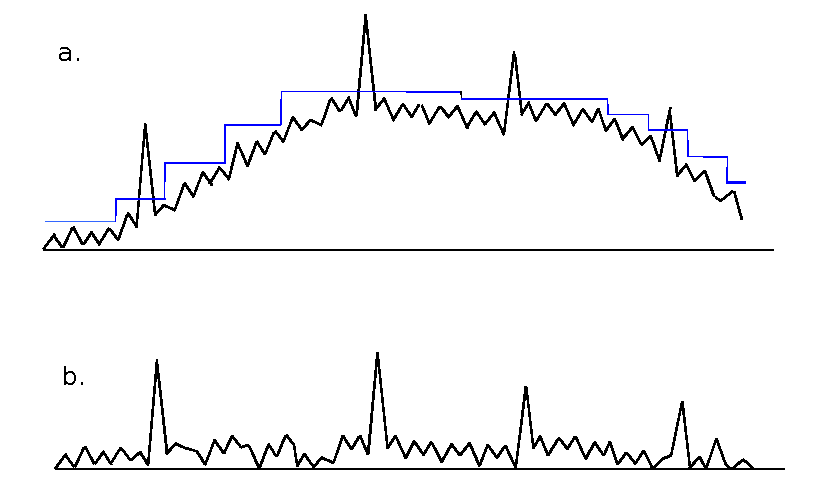
\includegraphics[width=4.16667in,height=\textheight]{figs/cfar-signal.pdf}
\caption{The signal level within one pulse window: a) before CFAR; b)
after CFAR}\label{fig:cube-cfar-signal}
}
\end{figure}

\begin{Shaded}
\begin{Highlighting}[numbers=left,,firstnumber=374,]
\OtherTok{fCFAR ::} \DataTypeTok{Range}\NormalTok{ (}\DataTypeTok{Window} \DataTypeTok{RealData}\NormalTok{) }\OtherTok{->} \DataTypeTok{Range}\NormalTok{ (}\DataTypeTok{Window} \DataTypeTok{RealData}\NormalTok{)}
\NormalTok{fCFAR rbins }\FunctionTok{=}\NormalTok{ V.farm41 (\textbackslash{}m }\OtherTok{->}\NormalTok{ V.farm31 (normCfa m)) md rbins lmv emv}
  \KeywordTok{where}
\NormalTok{    md  }\FunctionTok{=}\NormalTok{ V.farm11 (}\FunctionTok{logBase} \DecValTok{2} \FunctionTok{.}\NormalTok{ V.reduce }\FunctionTok{min}\NormalTok{) rbins}
\NormalTok{    emv }\FunctionTok{=}\NormalTok{ (V.fanoutn (nFFT }\FunctionTok{+} \DecValTok{1}\NormalTok{) dummy) }\FunctionTok{<++>}\NormalTok{ (V.farm11 aritMean neighbors)}
\NormalTok{    lmv }\FunctionTok{=}\NormalTok{ (V.drop }\DecValTok{2} \FunctionTok{$}\NormalTok{ V.farm11 aritMean neighbors) }\FunctionTok{<++>}\NormalTok{ (V.fanout dummy) }
    \CommentTok{-----------------------------------------------}
\NormalTok{    normCfa m a l e }\FunctionTok{=} \DecValTok{2} \FunctionTok{**}\NormalTok{ (}\DecValTok{5} \FunctionTok{+} \FunctionTok{logBase} \DecValTok{2}\NormalTok{ a }\FunctionTok{-} \FunctionTok{maximum}\NormalTok{ [l,e,m])}
\OtherTok{    aritMean ::} \DataTypeTok{Vector}\NormalTok{ (}\DataTypeTok{Vector} \DataTypeTok{RealData}\NormalTok{) }\OtherTok{->} \DataTypeTok{Vector} \DataTypeTok{RealData}
\NormalTok{    aritMean  }\FunctionTok{=}\NormalTok{ V.farm11 (}\FunctionTok{/}\NormalTok{n) }\FunctionTok{.}\NormalTok{ V.reduce addV }\FunctionTok{.}\NormalTok{ V.farm11 geomMean }\FunctionTok{.}\NormalTok{ V.group }\DecValTok{4}
\NormalTok{    geomMean  }\FunctionTok{=}\NormalTok{ V.farm11 (}\FunctionTok{logBase} \DecValTok{2} \FunctionTok{.}\NormalTok{ (}\FunctionTok{/}\DecValTok{4}\NormalTok{)) }\FunctionTok{.}\NormalTok{ V.reduce addV}
    \CommentTok{-----------------------------------------------}
\NormalTok{    dummy     }\FunctionTok{=}\NormalTok{ V.fanoutn nFFT }\FunctionTok{$}\NormalTok{ (}\FunctionTok{-}\NormalTok{maxFloat)}\FunctionTok{/}\NormalTok{n}
\NormalTok{    neighbors }\FunctionTok{=}\NormalTok{ V.stencil nFFT rbins}
    \CommentTok{-----------------------------------------------}
\NormalTok{    addV      }\FunctionTok{=}\NormalTok{ V.farm21 (}\FunctionTok{+}\NormalTok{)}
\NormalTok{    n         }\FunctionTok{=} \FunctionTok{fromIntegral}\NormalTok{ nFFT}
\end{Highlighting}
\end{Shaded}

\begin{longtable}[]{@{}lll@{}}
\toprule
Function & Original module & Package\tabularnewline
\midrule
\endhead
\texttt{farm}{[}\texttt{4}/\texttt{3}/\texttt{1}{]}\texttt{1},
\texttt{reduce}, \texttt{\textless{}++\textgreater{}}, &
\href{https://forsyde.github.io/forsyde-atom/api/ForSyDe-Atom-Skeleton-Vector.html}{\texttt{ForSyDe.Atom.Skeleton.Vector}}
& forsyde-atom\tabularnewline
\texttt{drop}, \texttt{fanout}, \texttt{fanoutn}, \texttt{stencil} &
&\tabularnewline
\texttt{comb11} &
\href{https://forsyde.github.io/forsyde-atom/api/ForSyDe-Atom-MoC-SY.html}{\texttt{ForSyDe.Atom.MoC.SY}}
& forsyde-atom\tabularnewline
\texttt{maxFloat} & ForSyDe.AESA.Coefs & aesa-atom\tabularnewline
\texttt{nb}, \texttt{nFFT} & \texttt{ForSyDe.AESA.Params} &
aesa-atom\tabularnewline
\bottomrule
\end{longtable}

The \(f_{CFAR}\) function itself can be described with the system of
eq.~\ref{eq:cfar}, where

\begin{itemize}
\item
  \(MD\) is the minimum value over all Doppler channels in a batch for a
  specific data channel and range bin.
\item
  \(EMV\) and \(LMV\) calculate the early and respectively late mean
  values from the neighboring range bins as a combination of geometric
  and arithmetic mean values.
\item
  \(eb\) and \(lb\) are the earliest bin, respectively latest bin for
  which the CFAR can be calculated as \(EMV\) and \(LMV\) require at
  least \(N_{FFT}\) bins + 1 guard bin before and respectively after the
  current bin. This phenomenon is also called the ``stencil halo'',
  which means that CFAR, as defined in eq.~\ref{eq:cfar} is applied only
  on \(N_b'=N_b-2N_{FFT}-2\) bins.
\item
  bins earlier than \(eb\), respectively later than \(lb\), are ingnored
  by the CFAR formula and therefore their respective EMV and LMV are
  replaced with the lowest representable value.
\item
  5 is added to the exponent of the CFAR equation to set the gain to 32
  (i.e.~with only noi se in the incoming video the output values will be
  32).
\end{itemize}

\begin{equation}\begin{aligned}&\left\{\begin{aligned}
  &CFAR(a_{ij})= 2^{(5 + \log_2 a_{ij}) - \max (EMV(a_{ij}),LMV(a_{ij}),MD(a_{ij}))}\\
  &EMV(a_{ij}) = \frac{1}{N}\sum_{k=0}^{N-1}\left(\log_2\left(\frac{1}{4}\sum_{l=0}^{3}a_{(i-2-4k-l)j}\right)\right)\\
  &LMV(a_{ij}) = \frac{1}{N}\sum_{k=0}^{N-1}\left(\log_2\left(\frac{1}{4}\sum_{l=0}^{3}a_{(i+2+4k+l)j}\right)\right)\\
  &MD(a_{ij})  = \log_{2}\left(\min_{k=1}^N(a_{ik})\right)
  \end{aligned}\right.\\
  &\qquad \forall i\in[eb,lb], j\in[1,N] \text{ where }\left\{
  \begin{aligned}
  &N = N_{FFT}\\
  &eb = N_{FFT} + 1\\
  &lb = N_b - N_{FFT} - 1\\
  \end{aligned}\right.
  \end{aligned}
\label{eq:cfar}\end{equation}

The first thing we calculate is the \(MD\) for each Doppler window
(row). For each row of \texttt{rbins} (i.e.~range bins of Doppler
windows) we look for the minimum value (\texttt{reduceV\ min}) and apply
the binary logarithm on it.

Another action performed over the matrix \texttt{rbins} is to form two
stencil ``cubes'' for EMV and LMV respectively, by gathering batches of
\(N_{FFT}\) Doppler windows like in eq.~\ref{eq:cfar-stencil}, computing
them like in eq.~\ref{eq:cfar-emv}.

\begin{equation}
  \stackrel{\mbox{rbins}}{
  \begin{bmatrix}
  a_{11} & a_{12} & \cdots & a_{1N_{FFT}} \\
  a_{21} & a_{22} & \cdots & a_{2N_{FFT}} \\
  \vdots & \vdots & \ddots & \vdots \\
  a_{N_b1} & a_{N_b2} & \cdots & a_{N_bN_{FFT}}
  \end{bmatrix}}
  \stackrel{\mathtt{stencil}}{\rightarrow}
  \stackrel{\mbox{neighbors}}{
  \begin{bmatrix}
  \begin{bmatrix}
  a_{11} & a_{12} & \cdots & a_{1N_{FFT}} \\
  \vdots & \vdots & \ddots & \vdots \\
  a_{N_{FFT}1} & a_{N_{FFT}2} & \cdots & a_{N_{FFT}N_{FFT}} \\
  \end{bmatrix}\\
  \begin{bmatrix}
  a_{21} & a_{22} & \cdots & a_{2N_{FFT}} \\
  \vdots & \vdots & \ddots & \vdots \\
  a_{(N_{FFT}+1)1} & a_{(N_{FFT}+1)2} & \cdots & a_{(N_{FFT}+1)N_{FFT}} \\
  \end{bmatrix}\\
  \vdots \\
  \begin{bmatrix}
  a_{(N_b-N_{FFT})1} & a_{(N_b-N_{FFT})2} & \cdots & a_{(N_b-N_{FFT})N_{FFT}}\\
  \vdots & \vdots & \ddots & \vdots \\
  a_{N_b1} & a_{N_b2} & \cdots & a_{N_bN_{FFT}}
  \end{bmatrix}
  \end{bmatrix}}
\label{eq:cfar-stencil}\end{equation}

Each one of these neighbors matrices will constitute the input data for
calculating the \(EMV\) and \(LMV\) for each Doppler window. \(EMV\) and
\(LMV\) are calculated by applying the mean function \texttt{arithMean}
over them, as shown (only for the window associated with the \(eb\) bin)
in eq.~\ref{eq:cfar-emv}. The resulting \texttt{emv} and \texttt{lmv}
matrices are padded with rows of the minimum representable value
\texttt{-maxFloat}, so that they align properly with \texttt{rbins} in
order to combine into the 2D farm/stencil defined at eq.~\ref{eq:cfar}.
Finally, \texttt{fCFAR} yields a matrix of normalized Doppler windows.
The resulting matrices are not transformed back into sample streams by
the parent process, but rather they are passed as single tokens
downstream to the INT stage, where they will be processed as such.

\begin{equation}\begin{aligned}
  &\begin{bmatrix}
  a_{11} & \cdots & a_{1N_{FFT}} \\
  \vdots  & \ddots & \vdots \\
  a_{N_{FFT}1}  & \cdots & a_{N_{FFT}N_{FFT}}
  \end{bmatrix}
  \stackrel{\mathtt{group}}{\rightarrow}
  \begin{bmatrix}
  \begin{bmatrix}
  a_{11} & \cdots & a_{1N_{FFT}} \\
  \vdots & \ddots & \vdots \\
  a_{41} & \cdots & a_{4N_{FFT}}
  \end{bmatrix}\\
  \vdots \\
  \begin{bmatrix}
  a_{(N_{FFT}-4)1}  & \cdots & a_{(N_{FFT}-4)N_{FFT}}\\
  \vdots & \ddots & \vdots \\
  a_{N_{FFT}1}  & \cdots & a_{N_{FFT}N_{FFT}}
  \end{bmatrix}
  \end{bmatrix}\\
  &\stackrel{\mathtt{farm(geomMean)}}{\rightarrow}
  \begin{bmatrix}
  \log_2\frac{1}{4}\sum_{i=1}^{4}a_{i1} & \cdots & \log_2\frac{1}{4}\sum_{i=1}^{4}a_{iN_{FFT}} \\
  \vdots & \ddots & \vdots \\
  \log_2\frac{1}{4}\sum_{i=N_{FFT}-4}^{N_{FFT}}a_{i1} & \cdots & \log_2\frac{1}{4}\sum_{i=N_{FFT}-4}^{N_{FFT}}a_{iN_{FFT}}
  \end{bmatrix}\\
  &\stackrel{\mathtt{(/N_{FFT})\circ reduce(+)}}{\rightarrow}
  \begin{bmatrix}
  EMV(a_{eb,1}) & \cdots & EMV(a_{eb,N_{FFT}}) 
  \end{bmatrix}
  \end{aligned}
\label{eq:cfar-emv}\end{equation}

\hypertarget{sec:cube-int-atom}{%
\paragraph{Integrator (INT)}\label{sec:cube-int-atom}}

During the last stage of the video processing chain each data sample of
the video cube is integrated against its 8 previous values using an
8-tap FIR filter, as suggested by the drawing in
Figure~\ref{fig:cube-int-cube-atom}.

\begin{Shaded}
\begin{Highlighting}[numbers=left,,firstnumber=523,]
\OtherTok{int ::} \DataTypeTok{Signal}\NormalTok{ (}\DataTypeTok{Beam}\NormalTok{ (}\DataTypeTok{Range}\NormalTok{ (}\DataTypeTok{Window} \DataTypeTok{RealData}\NormalTok{)))}
    \OtherTok{->} \DataTypeTok{Signal}\NormalTok{ (}\DataTypeTok{Beam}\NormalTok{ (}\DataTypeTok{Range}\NormalTok{ (}\DataTypeTok{Window} \DataTypeTok{RealData}\NormalTok{)))}
    \OtherTok{->} \DataTypeTok{Signal}\NormalTok{ (}\DataTypeTok{Beam}\NormalTok{ (}\DataTypeTok{Range}\NormalTok{ (}\DataTypeTok{Window} \DataTypeTok{RealData}\NormalTok{)))}
\NormalTok{int right left }\FunctionTok{=}\NormalTok{ firNet mkIntCoefs }\FunctionTok{$}\NormalTok{ SY.interleave right left}
\end{Highlighting}
\end{Shaded}

Before integrating though, the data from both the left and the right
channel need to be merged and interleaved. This is done by the process
\texttt{interleave} below, which is a convenient utility exported by the
SY library, hiding a domain interface. When considering only the data
structures, the \texttt{interleave} process can be regarded as an
up-sampler with the rate 2/1. When taking into consideration the size of
the entire data set (i.e.~token rates \(\times\) structure sizes
\(\times\) data size), we can easily see that the overall required
system bandwidth (ratio) remains the same between the PC and INT stages,
i.e.~\(\frac{2\times N_B \times N_{b} \times N_{FFT}\times \mathit{size}(\mathtt{RealData})}{N_B \times N_{b} \times N_{FFT}\times \mathit{size}(\mathtt{CpxData})}=1/1\).

\begin{longtable}[]{@{}lll@{}}
\toprule
\begin{minipage}[b]{0.30\columnwidth}\raggedright
Function\strut
\end{minipage} & \begin{minipage}[b]{0.36\columnwidth}\raggedright
Original module\strut
\end{minipage} & \begin{minipage}[b]{0.26\columnwidth}\raggedright
Package\strut
\end{minipage}\tabularnewline
\midrule
\endhead
\begin{minipage}[t]{0.30\columnwidth}\raggedright
\texttt{farm21},\texttt{farm11},\texttt{fanout}\strut
\end{minipage} & \begin{minipage}[t]{0.36\columnwidth}\raggedright
ForSyDe.Atom.Skeleton.Vector.Cube\strut
\end{minipage} & \begin{minipage}[t]{0.26\columnwidth}\raggedright
forsyde-atom-extensions\strut
\end{minipage}\tabularnewline
\begin{minipage}[t]{0.30\columnwidth}\raggedright
\texttt{fir\textquotesingle{}}\strut
\end{minipage} & \begin{minipage}[t]{0.36\columnwidth}\raggedright
ForSyDe.Atom.Skeleton.Vector.DSP\strut
\end{minipage} & \begin{minipage}[t]{0.26\columnwidth}\raggedright
forsyde-atom-extensions\strut
\end{minipage}\tabularnewline
\begin{minipage}[t]{0.30\columnwidth}\raggedright
\texttt{comb21},\texttt{comb11}, \texttt{delay},
\texttt{interleave}\strut
\end{minipage} & \begin{minipage}[t]{0.36\columnwidth}\raggedright
\href{https://forsyde.github.io/forsyde-atom/api/ForSyDe-Atom-MoC-SY.html}{\texttt{ForSyDe.Atom.MoC.SY}}\strut
\end{minipage} & \begin{minipage}[t]{0.26\columnwidth}\raggedright
forsyde-atom\strut
\end{minipage}\tabularnewline
\begin{minipage}[t]{0.30\columnwidth}\raggedright
\texttt{mkFirCoefs}\strut
\end{minipage} & \begin{minipage}[t]{0.36\columnwidth}\raggedright
ForSyDe.AESA.Coefs\strut
\end{minipage} & \begin{minipage}[t]{0.26\columnwidth}\raggedright
aesa-atom\strut
\end{minipage}\tabularnewline
\bottomrule
\end{longtable}

\begin{figure}
\hypertarget{fig:cube-int-cube-atom}{%
\centering
\includegraphics{figs/int-cube.pdf}
\caption{Integration on cubes of complex
samples}\label{fig:cube-int-cube-atom}
}
\end{figure}

\begin{figure}
\hypertarget{fig:cube-int-atom}{%
\centering
\includegraphics{figs/int-proc-atom.pdf}
\caption{INT network}\label{fig:cube-int-atom}
}
\end{figure}

The 8-tap FIR filter used for integration is also a moving average, but
as compared to the \texttt{fir} function used in
section~\ref{sec:cube-pc-atom}, the window slides in time domain,
i.e.~over streaming samples rather than over vector elements. To
instantiate a FIR system we use the \texttt{fir\textquotesingle{}}
skeleton provided by the ForSyDe-Atom DSP utility libraries, which
constructs the the well-recognizable FIR pattern in
Figure~\ref{fig:cube-int-net-atom}, i.e.~a recur-farm-reduce
composition. In order to do so, \texttt{fir\textquotesingle{}} needs to
know \emph{what} to fill this template with, thus we need to provide as
arguments its ``basic'' operations, which in our case are processes
operating on signals of matrices. In fact, \texttt{fir} itself is a
\emph{specialization} of the \texttt{fir\textquotesingle{}} skeleton,
which defines its basic operations as corresponding functions on
vectors. This feature derives from a powerful algebra of skeletons which
grants them both modularity, and the possibility to transform them into
semantically-equivalent forms, as we shall soon explore in
section~\ref{sec:refinement}.

\begin{Shaded}
\begin{Highlighting}[numbers=left,,firstnumber=564,]
\OtherTok{firNet ::} \DataTypeTok{Num}\NormalTok{ a }\OtherTok{=>} \DataTypeTok{Vector}\NormalTok{ a }\OtherTok{->} \DataTypeTok{SY.Signal}\NormalTok{ (}\DataTypeTok{Cube}\NormalTok{ a) }\OtherTok{->} \DataTypeTok{SY.Signal}\NormalTok{ (}\DataTypeTok{Cube}\NormalTok{ a)}
\NormalTok{firNet coefs }\FunctionTok{=}\NormalTok{ fir' addSC mulSC dlySC coefs}
  \KeywordTok{where}
\NormalTok{    addSC   }\FunctionTok{=}\NormalTok{ SY.comb21 (C.farm21 (}\FunctionTok{+}\NormalTok{))}
\NormalTok{    mulSC c }\FunctionTok{=}\NormalTok{ SY.comb11 (C.farm11 (}\FunctionTok{*}\NormalTok{c))}
\NormalTok{    dlySC   }\FunctionTok{=}\NormalTok{ SY.delay  (C.fanout }\DecValTok{0}\NormalTok{)}
\end{Highlighting}
\end{Shaded}

\hypertarget{system-process-network}{%
\subsubsection{System Process Network}\label{system-process-network}}

The AESA process network is formed by ``plugging in'' together all
components instantiated in the previous sections, and thus obtaining the
system description in Figure~\ref{fig:cube-aesa-atom}. We do not
transpose the output data, because the Doppler windows are the ones we
are interested in plotting as the innermost structures.

\begin{figure}
\hypertarget{fig:cube-aesa-atom}{%
\centering
\includegraphics{figs/aesa-proc-atom.pdf}
\caption{The AESA process network instance}\label{fig:cube-aesa-atom}
}
\end{figure}

\begin{Shaded}
\begin{Highlighting}[numbers=left,,firstnumber=580,]
\OtherTok{aesa ::} \DataTypeTok{Signal}\NormalTok{ (}\DataTypeTok{Antenna}\NormalTok{ (}\DataTypeTok{Window}\NormalTok{ (}\DataTypeTok{Range}  \DataTypeTok{CpxData}\NormalTok{ )))}
     \OtherTok{->} \DataTypeTok{Signal}\NormalTok{ (}\DataTypeTok{Beam}\NormalTok{    (}\DataTypeTok{Range}\NormalTok{  (}\DataTypeTok{Window} \DataTypeTok{RealData}\NormalTok{)))}
\NormalTok{aesa video }\FunctionTok{=}\NormalTok{ int rCfar lCfar}
  \KeywordTok{where}
\NormalTok{    rCfar }\FunctionTok{=}\NormalTok{ cfar }\FunctionTok{$}\NormalTok{ dfb oPc}
\NormalTok{    lCfar }\FunctionTok{=}\NormalTok{ cfar }\FunctionTok{$}\NormalTok{ dfb }\FunctionTok{$}\NormalTok{ overlap oPc}
\NormalTok{    oPc   }\FunctionTok{=}\NormalTok{ pc }\FunctionTok{$}\NormalTok{ dbf video}
\end{Highlighting}
\end{Shaded}

\hypertarget{sec:aesa-parameters}{%
\subsubsection{System Parameters}\label{sec:aesa-parameters}}

Here we define the size constants, for a simple test scenario provided
by Saab AB. The size \texttt{nA} can be inferred from the size of input
data and the vector operations.

\begin{Shaded}
\begin{Highlighting}[numbers=left,,firstnumber=6,]
\KeywordTok{module} \DataTypeTok{ForSyDe.AESA.Params} \KeywordTok{where}

\NormalTok{nA   }\FunctionTok{=}   \DecValTok{16}\OtherTok{ ::} \DataTypeTok{Int}
\NormalTok{nB   }\FunctionTok{=}    \DecValTok{8}\OtherTok{ ::} \DataTypeTok{Int}
\NormalTok{nb   }\FunctionTok{=} \DecValTok{1024}\OtherTok{ ::} \DataTypeTok{Int}
\NormalTok{nFFT }\FunctionTok{=}  \DecValTok{256}\OtherTok{ ::} \DataTypeTok{Int}
\NormalTok{nS   }\FunctionTok{=}    \DecValTok{8}\OtherTok{ ::} \DataTypeTok{Int} \CommentTok{-- 2^nS = nFFT; used for convenience}

\NormalTok{freqRadar  }\FunctionTok{=} \FloatTok{10e9}\OtherTok{ ::} \DataTypeTok{Float} \CommentTok{-- 10 Ghz X-band}
\NormalTok{waveLength }\FunctionTok{=} \FloatTok{3e8} \FunctionTok{/}\NormalTok{ freqRadar}
\NormalTok{dElements  }\FunctionTok{=}\NormalTok{ waveLength}\FunctionTok{/}\DecValTok{2}
\end{Highlighting}
\end{Shaded}

\hypertarget{sec:coefs-atom}{%
\subsubsection{Coefficient Generators}\label{sec:coefs-atom}}

Here we define the vectors of coefficients used throughout the AESA
design. We keep this module as independent as possible from the main
design and export the coefficients both as ForSyDe-Atom vectors but also
as Haskell native lists, so that other packages can make use of them,
without importing the whole ForSyDe-Atom chain.

\begin{Shaded}
\begin{Highlighting}[numbers=left,,firstnumber=8,]
\OtherTok{\{-# LANGUAGE PackageImports #-\}}
\KeywordTok{module} \DataTypeTok{ForSyDe.AESA.Coefs} \KeywordTok{where}
\end{Highlighting}
\end{Shaded}

\begin{Shaded}
\begin{Highlighting}[numbers=left,,firstnumber=11,]
\KeywordTok{import}\NormalTok{ "forsyde-atom-extensions" }\DataTypeTok{ForSyDe.Atom.Skeleton.Vector} \KeywordTok{as} \DataTypeTok{V}
\KeywordTok{import} \DataTypeTok{ForSyDe.Atom.Skeleton.Vector.Matrix} \KeywordTok{as} \DataTypeTok{M}
\KeywordTok{import} \DataTypeTok{ForSyDe.Atom.Skeleton.Vector.DSP}
\KeywordTok{import} \DataTypeTok{Data.Complex}
\end{Highlighting}
\end{Shaded}

The \texttt{mkBeamConst} generator creates a matrix of \(\alpha_{ij}\)
beam constants used in the digital beamforming stage
section~\ref{sec:dbf-atom}. These beam constants perform both phase
shift and tapering according to eq.~\ref{eq:beam-coef}, where \(c_k\)
performs tapering and \(\varphi_{kl}\) perform phase shifting. For
tapering we use a set of Taylor coefficients generated with our in-house
utility \texttt{taylor}. The phase shift shall be calculated according
to eq.~\ref{eq:beam-phase}, where \(d\) is the distance between the
antenna elements. \(\theta_l\) is the angle between the wave front of
the current beam and normal of the antenna elements and \(\lambda\) is
the wavelength of the pulse.

\begin{equation} \alpha_{kl}=c_k e^{j\varphi_{kl}},\ \forall k\in[0,N_A-1], l \in [0,N_B-1]\label{eq:beam-coef}\end{equation}

\begin{equation} \varphi_{kl}=\frac{(k-9.5)\cdot 2\pi\cdot d \sin\theta}{\lambda}\label{eq:beam-phase}\end{equation}

\begin{Shaded}
\begin{Highlighting}[numbers=left,,firstnumber=29,]
\OtherTok{mkBeamConsts ::} \DataTypeTok{RealFloat}\NormalTok{ a}
             \OtherTok{=>}\NormalTok{ a                  }\CommentTok{-- ^ distance between radar elements}
             \OtherTok{->}\NormalTok{ a                  }\CommentTok{-- ^ radar signal wavelength}
             \OtherTok{->} \DataTypeTok{Int}                \CommentTok{-- ^ Number of antenna elements}
             \OtherTok{->} \DataTypeTok{Int}                \CommentTok{-- ^ Number of resulting beams}
             \OtherTok{->} \DataTypeTok{Matrix}\NormalTok{ (}\DataTypeTok{Complex}\NormalTok{ a)}
\NormalTok{mkBeamConsts d lambda nA nB }\FunctionTok{=}\NormalTok{ M.farm21 mulScale taperingCf phaseShiftCf}
  \KeywordTok{where}
    \CommentTok{-- all coefficients are normalized, i.e. scaled with 1/nA' }
\NormalTok{    mulScale x y   }\FunctionTok{=}\NormalTok{ x }\FunctionTok{*}\NormalTok{ y }\FunctionTok{/}\NormalTok{ nA'}
    \CommentTok{-- tapering coefficients, c_k in Eq. (4)}
\NormalTok{    taperingCf     }\FunctionTok{=}\NormalTok{ V.farm11 (V.fanoutn nB) taylorCf}
    \CommentTok{-- phase shift coefficients, e^(j*phi_kl) in Eqs.(4) and (5)}
\NormalTok{    phaseShiftCf   }\FunctionTok{=}\NormalTok{ V.farm11 (\textbackslash{}k }\OtherTok{->}\NormalTok{ V.farm11 (mkCf k) thetas) antennaIxs}
\NormalTok{    mkCf k theta_l }\FunctionTok{=}\NormalTok{ cis }\FunctionTok{$}\NormalTok{ (k }\FunctionTok{-} \FloatTok{9.5}\NormalTok{) }\FunctionTok{*} \DecValTok{2} \FunctionTok{*} \FunctionTok{pi} \FunctionTok{*}\NormalTok{ d }\FunctionTok{*} \FunctionTok{sin}\NormalTok{ theta_l }\FunctionTok{/}\NormalTok{ lambda}
    \CommentTok{--------------}
    \CommentTok{-- Taylor series: nA real numbers; 4 nearly constant adjacent side lobes;}
    \CommentTok{-- peak sidelobe level of -30dB}
\NormalTok{    taylorCf }\FunctionTok{=}\NormalTok{ taylor nA }\DecValTok{4}\NormalTok{ (}\FunctionTok{-}\DecValTok{30}\NormalTok{)}
    \CommentTok{-- theta_l spanning nB angles from 0 to pi}
\NormalTok{    thetas   }\FunctionTok{=}\NormalTok{ V.farm11 (\textbackslash{}t }\OtherTok{->} \FunctionTok{pi/}\DecValTok{3} \FunctionTok{+}\NormalTok{ t }\FunctionTok{*}\NormalTok{ (}\FunctionTok{pi} \FunctionTok{-} \DecValTok{2}\FunctionTok{*pi/}\DecValTok{3}\NormalTok{)}\FunctionTok{/}\NormalTok{(nB'}\FunctionTok{-}\DecValTok{1}\NormalTok{)) beamIxs}
    \CommentTok{--------------}
\NormalTok{    nA'       }\FunctionTok{=} \FunctionTok{fromIntegral}\NormalTok{ nA}
\NormalTok{    nB'       }\FunctionTok{=} \FunctionTok{fromIntegral}\NormalTok{ nB}
\NormalTok{    antennaIxs }\FunctionTok{=}\NormalTok{ vector }\FunctionTok{$} \FunctionTok{map} \FunctionTok{realToFrac}\NormalTok{ [}\DecValTok{0}\FunctionTok{..}\NormalTok{nA}\FunctionTok{-}\DecValTok{1}\NormalTok{]}
\NormalTok{    beamIxs    }\FunctionTok{=}\NormalTok{ vector }\FunctionTok{$} \FunctionTok{map} \FunctionTok{realToFrac}\NormalTok{ [}\DecValTok{0}\FunctionTok{..}\NormalTok{nB}\FunctionTok{-}\DecValTok{1}\NormalTok{]}
\end{Highlighting}
\end{Shaded}

\begin{Shaded}
\begin{Highlighting}[numbers=left,,firstnumber=56,]
\CommentTok{-- Can be used without importing the ForSyDe.Atom libraries.}
\OtherTok{mkBeamConsts' ::} \DataTypeTok{RealFloat}\NormalTok{ a }\OtherTok{=>}\NormalTok{ a }\OtherTok{->}\NormalTok{ a}\OtherTok{->} \DataTypeTok{Int} \OtherTok{->} \DataTypeTok{Int} \OtherTok{->}\NormalTok{ [[}\DataTypeTok{Complex}\NormalTok{ a]]}
\NormalTok{mkBeamConsts' d l nA nB }\FunctionTok{=} \FunctionTok{map}\NormalTok{ fromVector }\FunctionTok{$}\NormalTok{ fromVector }\FunctionTok{$}\NormalTok{ mkBeamConsts d l nA nB}
\end{Highlighting}
\end{Shaded}

\begin{longtable}[]{@{}lll@{}}
\toprule
\begin{minipage}[b]{0.23\columnwidth}\raggedright
Function\strut
\end{minipage} & \begin{minipage}[b]{0.41\columnwidth}\raggedright
Original module\strut
\end{minipage} & \begin{minipage}[b]{0.28\columnwidth}\raggedright
Package\strut
\end{minipage}\tabularnewline
\midrule
\endhead
\begin{minipage}[t]{0.23\columnwidth}\raggedright
\texttt{farm11},\texttt{farm21}, \texttt{fanout},
(\texttt{from}-)\texttt{vector}\strut
\end{minipage} & \begin{minipage}[t]{0.41\columnwidth}\raggedright
\href{https://forsyde.github.io/forsyde-atom/api/ForSyDe-Atom-Skeleton-Vector.html}{\texttt{ForSyDe.Atom.Skeleton.Vector}}\strut
\end{minipage} & \begin{minipage}[t]{0.28\columnwidth}\raggedright
forsyde-atom\strut
\end{minipage}\tabularnewline
\begin{minipage}[t]{0.23\columnwidth}\raggedright
\texttt{taylor}\strut
\end{minipage} & \begin{minipage}[t]{0.41\columnwidth}\raggedright
\texttt{ForSyDe.Atom.Skeleton.Vector.DSP}\strut
\end{minipage} & \begin{minipage}[t]{0.28\columnwidth}\raggedright
forsyde-atom-extensions\strut
\end{minipage}\tabularnewline
\bottomrule
\end{longtable}

The \texttt{mkPcCoefs} generator for the FIR filter in
section~\ref{sec:pc-atom} is simply a \(n\)-tap Hanning window. It can
be changed according to the user requirements. All coefficients are
scaled with \(1/n\) so that the output does not overflow a possible
fixed point representation.

\begin{Shaded}
\begin{Highlighting}[numbers=left,,firstnumber=72,]
\OtherTok{mkPcCoefs ::} \DataTypeTok{Fractional}\NormalTok{ a }\OtherTok{=>} \DataTypeTok{Int} \OtherTok{->} \DataTypeTok{Vector}\NormalTok{ a}
\NormalTok{mkPcCoefs n }\FunctionTok{=}\NormalTok{ V.farm11 (\textbackslash{}a }\OtherTok{->} \FunctionTok{realToFrac}\NormalTok{ a }\FunctionTok{/} \FunctionTok{realToFrac}\NormalTok{ n) }\FunctionTok{$}\NormalTok{ hanning n}
\end{Highlighting}
\end{Shaded}

\begin{longtable}[]{@{}lll@{}}
\toprule
Function & Original module & Package\tabularnewline
\midrule
\endhead
\texttt{hanning} & \texttt{ForSyDe.Atom.Skeleton.Vector.DSP} &
forsyde-atom-extensions\tabularnewline
\bottomrule
\end{longtable}

\begin{Shaded}
\begin{Highlighting}[numbers=left,,firstnumber=79,]

\CommentTok{-- Can be used without importing the ForSyDe.Atom libraries.}
\OtherTok{mkPcCoefs' ::} \DataTypeTok{Fractional}\NormalTok{ a }\OtherTok{=>} \DataTypeTok{Int} \OtherTok{->}\NormalTok{ [a]}
\NormalTok{mkPcCoefs' n }\FunctionTok{=}\NormalTok{ fromVector }\FunctionTok{$}\NormalTok{ mkPcCoefs n}
\end{Highlighting}
\end{Shaded}

We use also a Hanning window to generate the complex weight coefficients
for decreasing the Doppler side lobes during DFB in
section~\ref{sec:dfb-atom}. This can be changed according to the user
requirements.

\begin{Shaded}
\begin{Highlighting}[numbers=left,,firstnumber=88,]
\OtherTok{mkWeightCoefs ::} \DataTypeTok{Fractional}\NormalTok{ a }\OtherTok{=>} \DataTypeTok{Int} \OtherTok{->} \DataTypeTok{Vector}\NormalTok{ a}
\NormalTok{mkWeightCoefs nFFT }\FunctionTok{=}\NormalTok{ V.farm11 }\FunctionTok{realToFrac} \FunctionTok{$}\NormalTok{ hanning nFFT}
\end{Highlighting}
\end{Shaded}

\begin{Shaded}
\begin{Highlighting}[numbers=left,,firstnumber=91,]
\CommentTok{-- Can be used without importing the ForSyDe.Atom libraries.}
\OtherTok{mkWeightCoefs' ::} \DataTypeTok{Fractional}\NormalTok{ a }\OtherTok{=>} \DataTypeTok{Int} \OtherTok{->}\NormalTok{ [a]}
\NormalTok{mkWeightCoefs' nFFT }\FunctionTok{=}\NormalTok{ fromVector }\FunctionTok{$}\NormalTok{ mkWeightCoefs nFFT}
\end{Highlighting}
\end{Shaded}

For the integrator FIR in section~\ref{sec:int-atom} we use a normalized
square window.

\begin{Shaded}
\begin{Highlighting}[numbers=left,,firstnumber=97,]
\OtherTok{mkIntCoefs ::} \DataTypeTok{Fractional}\NormalTok{ a }\OtherTok{=>} \DataTypeTok{Vector}\NormalTok{ a}
\NormalTok{mkIntCoefs }\FunctionTok{=}\NormalTok{ vector mkIntCoefs'}
\end{Highlighting}
\end{Shaded}

\begin{Shaded}
\begin{Highlighting}[numbers=left,,firstnumber=100,]
\CommentTok{-- Can be used without importing the ForSyDe.Atom libraries.}
\OtherTok{mkIntCoefs' ::} \DataTypeTok{Fractional}\NormalTok{ a }\OtherTok{=>}\NormalTok{ [a]}
\NormalTok{mkIntCoefs' }\FunctionTok{=}\NormalTok{ [}\DecValTok{1}\FunctionTok{/}\DecValTok{8}\NormalTok{,}\DecValTok{1}\FunctionTok{/}\DecValTok{8}\NormalTok{,}\DecValTok{1}\FunctionTok{/}\DecValTok{8}\NormalTok{,}\DecValTok{1}\FunctionTok{/}\DecValTok{8}\NormalTok{,}\DecValTok{1}\FunctionTok{/}\DecValTok{8}\NormalTok{,}\DecValTok{1}\FunctionTok{/}\DecValTok{8}\NormalTok{,}\DecValTok{1}\FunctionTok{/}\DecValTok{8}\NormalTok{,}\DecValTok{1}\FunctionTok{/}\DecValTok{8}\NormalTok{] }
\end{Highlighting}
\end{Shaded}

\begin{Shaded}
\begin{Highlighting}[numbers=left,,firstnumber=104,]
\CommentTok{-- The maximum floating point number representable in Haskell. }
\OtherTok{maxFloat ::} \DataTypeTok{Float}
\NormalTok{maxFloat }\FunctionTok{=}\NormalTok{ x}
 \KeywordTok{where}\NormalTok{ n }\FunctionTok{=} \FunctionTok{floatDigits}\NormalTok{ x}
\NormalTok{       b }\FunctionTok{=} \FunctionTok{floatRadix}\NormalTok{ x}
\NormalTok{       (_, u) }\FunctionTok{=} \FunctionTok{floatRange}\NormalTok{ x}
\NormalTok{       x }\FunctionTok{=} \FunctionTok{encodeFloat}\NormalTok{ (b}\FunctionTok{^}\NormalTok{n }\FunctionTok{-} \DecValTok{1}\NormalTok{) (u }\FunctionTok{-}\NormalTok{ n)}
\end{Highlighting}
\end{Shaded}

\hypertarget{sec:atom-sim}{%
\subsection{Model Simulation Against Test Data}\label{sec:atom-sim}}

As a first trial to validate that our AESA high-level model is ``sane'',
i.e.~is modeling the expected behavior, we test it against realistic
input data from an array of antennas detecting some \emph{known}
objects. For this we have provided a set of data generator and plotter
scripts, along with an executable binary created with the
\texttt{CubesAtom} module presented in section~\ref{sec:atom-network}.
Please read the project's \texttt{README} file on how to compile and run
the necessary software tools.

The input data generator script replicates a situation in which 13
distinct objects, either near each other or far apart, as seen in
tbl.~\ref{tbl:in-objects}, are drowned into -18dB worth of noise, and
then detected by the 16 AESA antenna elements (see
section~\ref{sec:aesa-parameters}). A zoomed snapshot of the generated
input data can be seen in Figure~\ref{fig:aesa-indata}.

In Figure~\ref{fig:aesa-odata-atom} a cube consisting of 8 beam (doppler
\(\times\) range) matrices from the AESA signal processing output is
shown. We can see the 13 objects detected with different intensities
accros the 8 beams. As they are all positioned at approximately the same
angle relative to the antenna
(i.e.~\(\frac{\pi}{3} + 2(\pi-\frac{2\pi}{3})/7\)) we can see the
maximum correlation values are reflected in beam 2.

\nopandoc{\begin{landscape}}

\begin{figure}
\hypertarget{fig:aesa-indata}{%
\centering
\includegraphics{figs/AESA_INPUT_C.pdf}
\caption{One input video cube with antenna data. Samples' absolute
values are plotted.}\label{fig:aesa-indata}
}
\end{figure}

\begin{figure}
\hypertarget{fig:aesa-odata-atom}{%
\centering
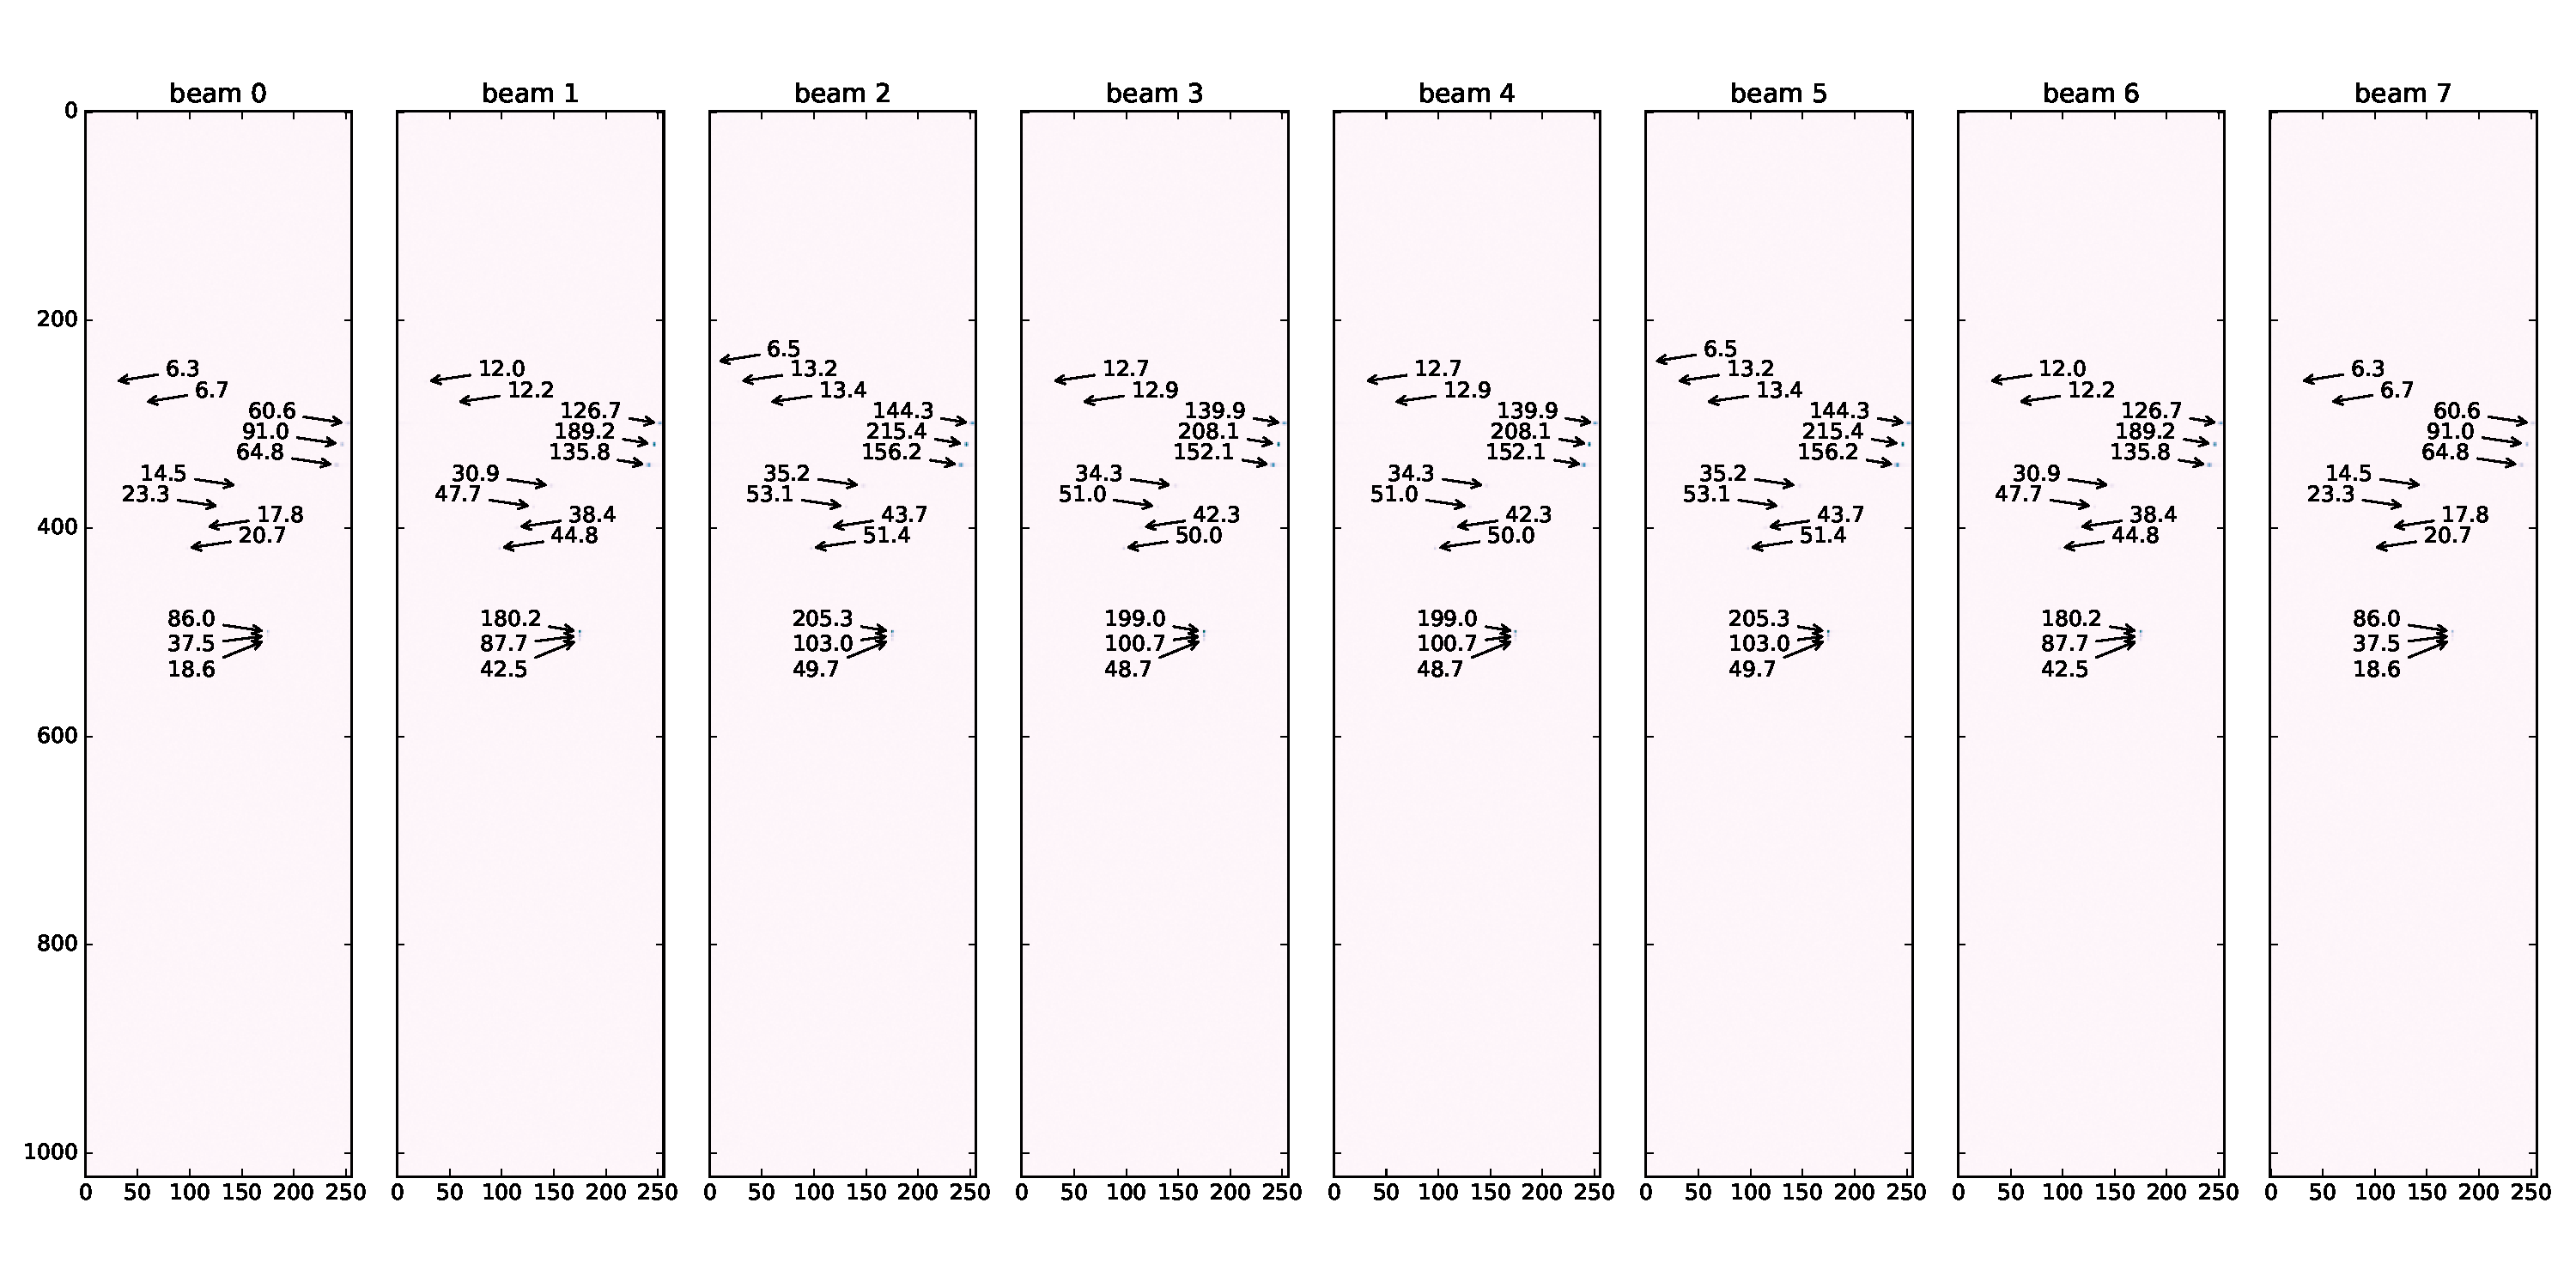
\includegraphics{figs/AESA_OUT_C.pdf}
\caption{One output cube with radar data.}\label{fig:aesa-odata-atom}
}
\end{figure}

\nopandoc{\end{landscape}}

\hypertarget{tbl:in-objects}{}
\begin{longtable}[]{@{}rrcrr@{}}
\caption{\label{tbl:in-objects}Objects reflected in the generated AESA
indata}\tabularnewline
\toprule
\# & Distance (m) & Angle (\(\theta\)) & Rel. Speed (m/s) & Rel.
Power\tabularnewline
\midrule
\endfirsthead
\toprule
\# & Distance (m) & Angle (\(\theta\)) & Rel. Speed (m/s) & Rel.
Power\tabularnewline
\midrule
\endhead
1 & 12e3 & \(\frac{\pi}{3} + 2(\pi-\frac{2\pi}{3})/7\) & 0.94 &
-6\tabularnewline
2 & 13e3 & \(\frac{\pi}{3} + 2(\pi-\frac{2\pi}{3})/7\) & 5 \(\cdot\)
0.94 & -6\tabularnewline
3 & 14e3 & \(\frac{\pi}{3} + 2(\pi-\frac{2\pi}{3})/7\) & 10 \(\cdot\)
0.94 & -6\tabularnewline
4 & 15e3 & \(\frac{\pi}{3} + 2(\pi-\frac{2\pi}{3})/7\) & -0.94 &
-2\tabularnewline
5 & 16e3 & \(\frac{\pi}{3} + 2(\pi-\frac{2\pi}{3})/7\) & -2 \(\cdot\)
0.94 & -2\tabularnewline
6 & 17e3 & \(\frac{\pi}{3} + 2(\pi-\frac{2\pi}{3})/7\) & -3 \(\cdot\)
0.94 & -2\tabularnewline
7 & 18e3 & \(\frac{\pi}{3} + 2(\pi-\frac{2\pi}{3})/7\) & -20 \(\cdot\)
0.94 & -4\tabularnewline
8 & 19e3 & \(\frac{\pi}{3} + 2(\pi-\frac{2\pi}{3})/7\) & -23 \(\cdot\)
0.94 & -4\tabularnewline
9 & 20e3 & \(\frac{\pi}{3} + 2(\pi-\frac{2\pi}{3})/7\) & -26 \(\cdot\)
0.94 & -4\tabularnewline
10 & 21e3 & \(\frac{\pi}{3} + 2(\pi-\frac{2\pi}{3})/7\) & -29 \(\cdot\)
0.94 & -4\tabularnewline
11 & 25e3 & \(\frac{\pi}{3} + 2(\pi-\frac{2\pi}{3})/7\) & -15 \(\cdot\)
0.94 & -2\tabularnewline
12 & 25.4e3 & \(\frac{\pi}{3} + 2.1(\pi-\frac{2\pi}{3})/7\) & -15
\(\cdot\) 0.94 & -4\tabularnewline
13 & 25.2e3 & \(\frac{\pi}{3} + 2.2(\pi-\frac{2\pi}{3})/7\) & -15
\(\cdot\) 0.94 & -3\tabularnewline
\bottomrule
\end{longtable}

\clearpage

\hypertarget{sec:shallow}{%
\section{Model Implementations in ForSyDe-Shallow}\label{sec:shallow}}

\href{https://forsyde.github.io/forsyde-shallow/}{ForSyDe-Shallow} is
the flagship and the oldest modeling language of the ForSyDe methodology
(Sander and Jantsch \protect\hyperlink{ref-sander-2004}{2004}). It is a
domain specific language (DSL) shallow-embedded into the functional
programming language Haskell and uses the host's type system, lazy
evaluation mechanisms and the concept of higher-order functions to
describe the formal modeling framework defined by ForSyDe.

As a first exercise we present a rather naïve model the AESA application
in ForSyDe-Shallow which mainly ``translates'' specification model as
given and presented in Figure~\ref{fig:video-chain-spec} into
ForSyDe-Haskell. We gradually build the designer's mindset and introduce
modeling concepts while we parse the source code of the ForSyDe model.
The model file is found at
\texttt{\textless{}root\textgreater{}/src/ForSyDe/Shallow/AESA.lhs} and
can be imported as a generic library (e.g.~in the interpreter session).

\hypertarget{sec:atom-network}{%
\subsection{The High-Level Model}\label{sec:atom-network}}

This section presents a high-level behavioral model of the AESA signal
processing chain presented in section~\ref{sec:video-chain-spec}, which
is, in any circumstance, \emph{not} the only modeling alternative, but
rather shows an intuitive and didactic way to tackle the challenge of
translating the \emph{textual} specifications into an \emph{executable}
ForSyDe specification. While most design choices are driven by the
ambition to introduce the new modeling concepts presented in
section~\ref{sec:crash-atom}, they can be justified by the need to
capture the essential behavioral properties in a formal way, in order to
be exploitable in future stages of a design flow towards efficient
implementations. The main design approach is to exploit the relative
independence between each data path associated with each antenna element
or beam, and to model these paths as skeletons (e.g.~farms) of (chains
of) processes. Each design decision will infer a re-partitioning of the
indata cubes between the time/causality and space dimensions following
the design patters depicted in Figure~\ref{fig:atom-layers}, namely:

\begin{itemize}
\item
  \emph{skeletons of processes} which: 1) express parallelism at the
  process level; 2) depicts processes as operating on elementary streams
  of data, e.g.~originating from each antenna element in particular, and
  skeletons as the structured interactions between these streams; 3)
  expose a fine-grained modular view allowing to quantify the potential
  for \emph{load distribution}, since each ``operation'' (i.e.~process)
  clearly captures the aspect of precedence constraints.
\item
  \emph{process of skeletons} which : 1) express parallelism at the
  datum level; 2) depicts processes as operating on structures of data
  (e.g.~vectors, matrices or cubes); 3) expose a monolithic view of
  processes where precedence constraints are expressed ``outside'' of
  the algorithm, and where the algorithm itself expresses potential for
  \emph{data parallelism}.
\end{itemize}

The code for this section is written in the following module, see
section~\ref{sec:usage} on how to use it:

\begin{Shaded}
\begin{Highlighting}[numbers=left,,firstnumber=33,]
\OtherTok{\{-# LANGUAGE PackageImports #-\}} \CommentTok{-- allows explicit import of modules from custom}
                                \CommentTok{-- libraries instead of standard ones. Will be taken}
                                \CommentTok{-- out once the extensions are merged upstream.}
\KeywordTok{module} \DataTypeTok{ForSyDe.AESA.StreamsAtom} \KeywordTok{where}
\end{Highlighting}
\end{Shaded}

\hypertarget{imported-libraries}{%
\subsubsection{Imported Libraries}\label{imported-libraries}}

As the AESA application uses complex numbers, we use Haskell's
\href{http://hackage.haskell.org/package/base/docs/Data-Complex.html}{\texttt{Complex}}
type.

\begin{Shaded}
\begin{Highlighting}[numbers=left,,firstnumber=43,]
\KeywordTok{import} \DataTypeTok{Data.Complex}
\end{Highlighting}
\end{Shaded}

For describing streaming behavior of the application our design will use
a heterogeneous approach, using a combination of \emph{synchronous
reactive (SY)} processes (Lee and Seshia
(\protect\hyperlink{ref-leeseshia-15}{2016}),Benveniste et al.
(\protect\hyperlink{ref-Benveniste03}{2003})), where the main assumption
is that all events in the system are synchronized; and \emph{synchronous
data flow (SDF)} processes (Lee and Seshia
(\protect\hyperlink{ref-leeseshia-15}{2016}),Lee and Parks
(\protect\hyperlink{ref-lee95}{1995})), where the temporal behavior is
formulated in terms of partial order constraints between events. We
import the
\href{https://forsyde.github.io/forsyde-atom/api/ForSyDe-Atom-MoC-SY.html}{\texttt{SY}}
and
\href{https://forsyde.github.io/forsyde-atom/api/ForSyDe-Atom-MoC-SDF.html}{\texttt{SDF}}
libraries described in the
\emph{\href{https://forsyde.github.io/forsyde-atom/api/ForSyDe-Atom-MoC.html}{MoC}
layer}, see (Ungureanu and Sander
\protect\hyperlink{ref-ungureanu17}{2017}), using an appropriate alias
for each.

\begin{Shaded}
\begin{Highlighting}[numbers=left,,firstnumber=57,]
\KeywordTok{import}\NormalTok{ "forsyde-atom-extensions" }\DataTypeTok{ForSyDe.Atom.MoC.SY}  \KeywordTok{as} \DataTypeTok{SY}
\KeywordTok{import}\NormalTok{ "forsyde-atom-extensions" }\DataTypeTok{ForSyDe.Atom.MoC.SDF} \KeywordTok{as} \DataTypeTok{SDF}
\end{Highlighting}
\end{Shaded}

For describing parallel operations on data we use algorithmic skeletons
(Fischer, Gorlatch, and Bischof
(\protect\hyperlink{ref-Fischer-2003}{2003}),Skillicorn
(\protect\hyperlink{ref-skillicorn05}{2005})), formulated on
ForSyDe-Atom's in-house
\href{http://hackage.haskell.org/package/forsyde-shallow/docs/ForSyDe-Shallow-Core-Vector.html}{\texttt{Vector}}
data type, which is a shallow, lazy-evaluated implementation of
unbounded arrays, ideal for early design validation. Although dependent,
bounded, and even boxed (i.e.~memory-mapped) alternatives exist, such as
\href{http://hackage.haskell.org/package/parameterized-data/docs/Data-Param-FSVec.html}{\texttt{FSVec}}
or REPA \href{http://hackage.haskell.org/package/repa}{\texttt{Array}}s,
for the scope of this project the functional validation and (by-hand)
requirement analysis on the properties of skeletons will suffice. We
also import the \texttt{Matrix} and \texttt{Cube} utility libraries
which contain type synonyms for nested \texttt{Vector}s along with their
derived skeletons, as well a \texttt{DSP} which contain commonly used
DSP blocks defined in terms of vector skeletons.

\begin{Shaded}
\begin{Highlighting}[numbers=left,,firstnumber=74,]
\KeywordTok{import}\NormalTok{ "forsyde-atom-extensions" }\DataTypeTok{ForSyDe.Atom.Skeleton.Vector}        \KeywordTok{as} \DataTypeTok{V}
\KeywordTok{import}\NormalTok{ "forsyde-atom-extensions" }\DataTypeTok{ForSyDe.Atom.Skeleton.Vector.Matrix} \KeywordTok{as} \DataTypeTok{M}
\KeywordTok{import}\NormalTok{ "forsyde-atom-extensions" }\DataTypeTok{ForSyDe.Atom.Skeleton.Vector.DSP}
\end{Highlighting}
\end{Shaded}

Finally, we import the local project module defining different
coefficients for the AESA algorithms, presented in detail in
section~\ref{sec:coefs-atom}.

\begin{Shaded}
\begin{Highlighting}[numbers=left,,firstnumber=81,]
\KeywordTok{import} \DataTypeTok{ForSyDe.AESA.Coefs}
\end{Highlighting}
\end{Shaded}

\hypertarget{sec:aliases-shallow}{%
\subsubsection{Type Aliases and Constants}\label{sec:aliases-shallow}}

The system parameters are integer constants defining the size of the
application. For a simple test scenario provided by Saab AB, we have
bundled these parameters in the following module, and we shall use their
variable names throughout the whole report:

\begin{Shaded}
\begin{Highlighting}[numbers=left,,firstnumber=89,]
\KeywordTok{import} \DataTypeTok{ForSyDe.AESA.Params}
\end{Highlighting}
\end{Shaded}

For ease of documentation we will be using type synonyms (aliases) for
all types and structures throughout this design:

\begin{itemize}
\item
  \texttt{Antenna} denotes a vector container for the antenna elements.
  Its length is equal to the number of antennas in the radar \(N_A\).
\item
  After Digital Beamforming (DBF), the antenna elements are transformed
  into \(N_B\) beams, thus we associate the \texttt{Beam} alias for the
  vector container wrapping those beams.
\item
  \texttt{Range} is a vector container for range bins. All antennas have
  the same number of range bins \(N_b\), rendering each
  \(\text{Antenna} \times \text{Range}\) a perfect matrix of samples for
  every pulse.
\item
  \texttt{Window} stands for a Doppler window of \(N_{FFT}\) pulses.
\end{itemize}

\begin{Shaded}
\begin{Highlighting}[numbers=left,,firstnumber=107,]
\KeywordTok{type} \DataTypeTok{Antenna}     \FunctionTok{=} \DataTypeTok{Vector} \CommentTok{-- length: nA}
\KeywordTok{type} \DataTypeTok{Beam}        \FunctionTok{=} \DataTypeTok{Vector} \CommentTok{-- length: nB}
\KeywordTok{type} \DataTypeTok{Range}       \FunctionTok{=} \DataTypeTok{Vector} \CommentTok{-- length: nb}
\KeywordTok{type} \DataTypeTok{Window}      \FunctionTok{=} \DataTypeTok{Vector} \CommentTok{-- length: nFFT}
\end{Highlighting}
\end{Shaded}

Finally we provide two aliases for the basic Haskell data types used in
the system, to stay consistent with the application specification.

\begin{Shaded}
\begin{Highlighting}[numbers=left,,firstnumber=115,]
\KeywordTok{type} \DataTypeTok{CpxData}  \FunctionTok{=} \DataTypeTok{Complex} \DataTypeTok{Float}
\KeywordTok{type} \DataTypeTok{RealData} \FunctionTok{=} \DataTypeTok{Float}
\end{Highlighting}
\end{Shaded}

\hypertarget{video-processing-stages}{%
\subsubsection{Video Processing Stages}\label{video-processing-stages}}

In this section we follow each stage described in
section~\ref{sec:video-chain-spec}, and exploit the initial assumption
on the order of events stating: \emph{``For each antenna the data
arrives \emph{pulse by pulse}, and each pulse arrives \emph{range bin by
range bin}. This happens \emph{for all antennas in parallel}, and all
complex samples are synchronized with the same sampling rate, e.g.~of
the A/D converter.''}

This allows us to ``unroll'' the indata video cubes into \(N_A\)
parallel synchronous streams, each stream being able to be processed as
soon as it contains enough data. This unrolling is depicted in
Figure~\ref{fig:cube-unrolling} as streaming the pulses as soon as they
arrive: range bin by range bin. We say that we partition the data
\emph{in time} rather than \emph{in space}, which is a more appropriate
partition judging by the assumption above.

\begin{figure}
\hypertarget{fig:cube-unrolling}{%
\centering
\includegraphics{figs/cube-unrolling.pdf}
\caption{Video cube unrolling}\label{fig:cube-unrolling}
}
\end{figure}

\hypertarget{sec:dbf-atom}{%
\paragraph{Digital Beamforming (DBF)}\label{sec:dbf-atom}}

The DBF receives complex in data, from \(N_A\) antenna elements and
forms \(N_B\) simultaneous receiver beams, or ``listening directions'',
by summing individually phase-shifted in data signals from all elements.
Depicted from a streaming point of view, DBF would like in
Figure~\ref{fig:dbf-samp}.

\suppressfloats

\begin{figure}
\hypertarget{fig:dbf-samp}{%
\centering
\includegraphics{figs/dbf-samp.pdf}
\caption{Digital Beam Forming on streams of complex
samples}\label{fig:dbf-samp}
}
\end{figure}

As can be seen in Figure~\ref{fig:dbf-samp}, a beam can be formed
\emph{as soon as} all antennas have produced a complex sample. The
parallel streams of data coming from each antenna element are
represented as a \emph{vector of synchronous (SY) signals}, i.e.~vector
of signals where each event is synchronous with each other. This allows
us to depict the dataflow interaction between the streams during digital
beamforming as the process network in Figure~\ref{fig:dbf-net-atom},
where an \(\oplus\) represents a combinational process
\href{https://forsyde.github.io/forsyde-atom/api/ForSyDe-Atom-MoC.html\#v:comb22}{\texttt{comb}}.

\suppressfloats

\begin{figure}
\hypertarget{fig:dbf-net-atom}{%
\centering
\includegraphics{figs/dbf-net-atom.pdf}
\caption{DBF network}\label{fig:dbf-net-atom}
}
\end{figure}

\begin{Shaded}
\begin{Highlighting}[numbers=left,,firstnumber=157,]
\OtherTok{dbf ::} \DataTypeTok{Antenna}\NormalTok{ (}\DataTypeTok{SY.Signal} \DataTypeTok{CpxData}\NormalTok{)}
    \OtherTok{->} \DataTypeTok{Beam}\NormalTok{    (}\DataTypeTok{SY.Signal} \DataTypeTok{CpxData}\NormalTok{)}
\NormalTok{dbf antennaSigs }\FunctionTok{=}\NormalTok{ beamSigs}
  \KeywordTok{where}
\NormalTok{    beamSigs   }\FunctionTok{=}\NormalTok{ V.reduce (V.farm21 (SY.comb21 (}\FunctionTok{+}\NormalTok{))) beamMatrix}
\NormalTok{    beamMatrix }\FunctionTok{=}\NormalTok{ M.farm21 (\textbackslash{}c }\OtherTok{->}\NormalTok{ SY.comb11 (}\FunctionTok{*}\NormalTok{c)) beamConsts sigMatrix}
\NormalTok{    sigMatrix  }\FunctionTok{=}\NormalTok{ V.farm11 V.fanout antennaSigs}
\NormalTok{    beamConsts }\FunctionTok{=}\NormalTok{ mkBeamConsts dElements waveLength nA}\OtherTok{ nB ::} \DataTypeTok{Matrix} \DataTypeTok{CpxData}
\end{Highlighting}
\end{Shaded}

\begin{longtable}[]{@{}lll@{}}
\toprule
Function & Original module & Package\tabularnewline
\midrule
\endhead
\texttt{farm11}, \texttt{reduce}, \texttt{length} &
\href{https://forsyde.github.io/forsyde-atom/api/ForSyDe-Atom-Skeleton-Vector.html}{\texttt{ForSyDe.Atom.Skeleton.Vector}}
& forsyde-atom\tabularnewline
\texttt{farm21} & \texttt{ForSyDe.Atom.Skeleton.Vector.Matrix} &
forsyde-atom-extensions\tabularnewline
\texttt{comb11}, \texttt{comb21} &
\href{https://forsyde.github.io/forsyde-atom/api/ForSyDe-Atom-MoC-SY.html}{\texttt{ForSyDe.Atom.MoC.SY}}
& forsyde-atom\tabularnewline
\texttt{mkBeamConsts} & \texttt{ForSyDe.AESA.Coefs} &
aesa-atom\tabularnewline
\texttt{dElements}, \texttt{waveLenth}, \texttt{nA}, \texttt{nB} &
\texttt{ForSyDe.AESA.Params} & aesa-atom\tabularnewline
\bottomrule
\end{longtable}

\suppressfloats

The previous code listing, depicted in Figure~\ref{fig:dbf-net-atom}, is
actually showing the ``internals'' of a matrix-vector dot
product{[}\^{}dotMatMat{]}. However, the elementary operations, instead
of regular arithmetic operations \(\times\) and \(+\), are
\emph{processes} applying these operations on SY streams. As such, the
\texttt{fanout} skeleton distributes one signal to a whole row
(i.e.~vector) of processes, the matrix \texttt{farm} applies pair-wise a
matrix of partially applied processes on this matrix of signals, and
\texttt{reduce} creates a reduction network of binary processes
pair-wise applying the function \(+\) on all events in signals.
Practically the DBF network transforms \(N_A\) synchronous signals
originating from each antenna element into \(N_B\) synchronous signals
for each beam. The internal structure of this transformation exposes
multiple degrees of potential distribution on parallel synchronous
resources.

The table above gives some pointers where to look for additional
documentation of each imported function. The formula to generate the
beam constants \texttt{mkBeamConsts} is presented later in
section~\ref{sec:atom-coefs}.

\hypertarget{sec:pc-atom}{%
\paragraph{Pulse Compression (PC)}\label{sec:pc-atom}}

In this stage the received echo of the modulated pulse, i.e.~the
information contained by the range bins, is passed through a matched
filter for decoding their modulation. This essentially applies a sliding
window, or a moving average (MAV) on the range bin samples.

\begin{figure}
\hypertarget{fig:pc-samp}{%
\centering
\includegraphics{figs/pc-samp.pdf}
\caption{Pulse Compression on streams of complex
samples}\label{fig:pc-samp}
}
\end{figure}

In Figure~\ref{fig:pc-samp} we can see that, in order to apply the MAV
algorithm on all the range bins of every pulse, we need to accumulate
\(N_b\) samples and process them in batches. Intuitively this can be
done by processing each beam with a \emph{synchronous dataflow} (SDF)
actor which, with each firing, consumes \(N_b\) samples and produces
\(N_b\) samples. Note that at this stage of modeling we value intuition
and the capturing of the right application properties rather than
efficiency. We will tackle this problem later in the design stages (see
section~\ref{sec:refinement}) where we will try to transform the model
toward more ``efficient'' implementation models (with respect to some
constraint, e.g.~throughput) which preserve these behavioral properties.

\begin{figure}
\hypertarget{fig:pc-proc-atom}{%
\centering
\includegraphics{figs/pc-proc-atom.pdf}
\caption{PC stage process}\label{fig:pc-proc-atom}
}
\end{figure}

\begin{Shaded}
\begin{Highlighting}[numbers=left,,firstnumber=213,]
\OtherTok{pc ::} \DataTypeTok{Beam}\NormalTok{ ( }\DataTypeTok{SY.Signal} \DataTypeTok{CpxData}\NormalTok{)}
   \OtherTok{->} \DataTypeTok{Beam}\NormalTok{ (}\DataTypeTok{SDF.Signal} \DataTypeTok{CpxData}\NormalTok{)}
\NormalTok{pc }\FunctionTok{=}\NormalTok{ V.farm11 (procPC }\FunctionTok{.}\NormalTok{ SY.toSDF)}
\end{Highlighting}
\end{Shaded}

\begin{longtable}[]{@{}lll@{}}
\toprule
Function & Original module & Package\tabularnewline
\midrule
\endhead
\texttt{farm11} &
\href{https://forsyde.github.io/forsyde-atom/api/ForSyDe-Atom-Skeleton-Vector.html}{\texttt{ForSyDe.Atom.Skeleton.Vector}}
& forsyde-atom\tabularnewline
\texttt{toSDF} &
\href{https://forsyde.github.io/forsyde-atom/api/ForSyDe-Atom-MoC-SY.html}{\texttt{ForSyDe.Atom.MoC.SY}}
& forsyde-atom\tabularnewline
\texttt{comb11} &
\href{https://forsyde.github.io/forsyde-atom/api/ForSyDe-Atom-MoC-SDF.html}{\texttt{ForSyDe.Atom.MoC.SDF}}
& forsyde-atom\tabularnewline
\texttt{fir} & \texttt{ForSyDe.Atom.Skeleton.Vector.DSP} &
forsyde-atom-extensions\tabularnewline
\texttt{mkPcCoefs} & \texttt{ForSyDe.AESA.Coefs} &
aesa-atom\tabularnewline
\texttt{nb} & \texttt{ForSyDe.AESA.Params} & aesa-atom\tabularnewline
\bottomrule
\end{longtable}

Following the reasoning above, we instantiate the PC video processing
stage as a \texttt{farm} of SDF processes \texttt{procPC} as depicted in
Figure~\ref{fig:pc-proc-atom}. Notice that before being able to apply
the SDF actors we need to translate the SY signals yielded by the DBF
stage into SDF signals. This is done by the \texttt{toSDF} interface
which is an injective mapping from the (timed) domain of a SY MoC tag
system, to the (untimed) codomain of a SDF MoC tag system. For more on
tag systems please consult (Lee and Sangiovanni-Vincentelli
\protect\hyperlink{ref-lee98}{1998}).

\begin{Shaded}
\begin{Highlighting}[numbers=left,,firstnumber=233,]
\OtherTok{procPC ::} \DataTypeTok{Fractional}\NormalTok{ a }\OtherTok{=>} \DataTypeTok{SDF.Signal}\NormalTok{ a }\OtherTok{->} \DataTypeTok{SDF.Signal}\NormalTok{ a }
\NormalTok{procPC }\FunctionTok{=}\NormalTok{ SDF.comb11 (nb, nb, V.fromVector }\FunctionTok{.}\NormalTok{ fir (mkPcCoefs }\DecValTok{5}\NormalTok{) }\FunctionTok{.}\NormalTok{ V.vector)}
\end{Highlighting}
\end{Shaded}

The \texttt{procPC} actor consumes and produces \texttt{nb} tokens each
firing, forms a \texttt{Vector} from these tokens, and applies the
\texttt{fir} skeleton on these vectors (which computes the MAV if
considering vectors). The \texttt{fir} skeleton is a utility formulated
in terms of primitive skeletons (i.e.~\texttt{map} and \texttt{reduce})
on numbers, i.e.~lifting arithmetic functions. We will study this
skeleton later in this report and for now we take it ``for granted'', as
conveniently provided by the \texttt{DSP} utility library. Also notice
that the type signature for \texttt{procPC} is left polymorphic as to be
more convenient later when we formulate properties over it.

\hypertarget{sec:ct-atom}{%
\paragraph{Corner Turn (CT)}\label{sec:ct-atom}}

In order to be able to calculate the Doppler channels further in the
processing pipeline, during a CT, a rearrangement of data must be
performed between functions that process data in ``different''
directions, e.g.~range and pulse. This rearrangement is called corner
turn. We make use of the knowledge that for each beam samples arrive in
order, one range bin at a time, in the direction of consumption
suggested in Figure~\ref{fig:ct-samp}, and ``fill back in'' the video
cube in the direction of production. In order to maximize the efficiency
of the AESA processing the datapath is split into two concurrent
processing channels with 50\% overlapped data, as shown in
Figure~\ref{fig:ct-cube}.

\begin{figure}
\hypertarget{fig:ct-samp}{%
\centering
\includegraphics{figs/ct-samp.pdf}
\caption{Building matrices of complex samples during
CT}\label{fig:ct-samp}
}
\end{figure}

\begin{figure}
\hypertarget{fig:ct-cube}{%
\centering
\includegraphics{figs/ct-cube.pdf}
\caption{Concurrent processing on 50\% overlapped
data}\label{fig:ct-cube}
}
\end{figure}

Our CT network thus maps on each beam signal a corner turn process
which, under the SDF execution semantics, consumes \(N_{FFT}\times N_b\)
ordered samples, interprets them as a matrix, transposes this matrix,
and produces \(N_b\times N_{FFT}\) samples ordered in the direction
suggested in Figure~\ref{fig:ct-samp}. In order to achieve 50\%
overlapping between the two output channels, the left one needs to be
``delayed'' with a prefix signal equivalent to half a video cube. In
this case that prefix is formed of \(\frac{N_b \times N_{FFT}}{2}\)
complex zeroes on each beam path. This way, whatever input arrives from
the PC stage, will be observed at the left channel only after
\(N_{FFT}/2\) samples.

\begin{Shaded}
\begin{Highlighting}[numbers=left,,firstnumber=271,]
\OtherTok{ct ::} \DataTypeTok{Beam}\NormalTok{ (}\DataTypeTok{SDF.Signal} \DataTypeTok{CpxData}\NormalTok{)}
   \OtherTok{->}\NormalTok{ (}\DataTypeTok{Beam}\NormalTok{ (}\DataTypeTok{SDF.Signal} \DataTypeTok{CpxData}\NormalTok{),}
       \DataTypeTok{Beam}\NormalTok{ (}\DataTypeTok{SDF.Signal} \DataTypeTok{CpxData}\NormalTok{))}
\NormalTok{ct }\FunctionTok{=}\NormalTok{ V.farm12 procCT}

\OtherTok{procCT ::} \DataTypeTok{Num}\NormalTok{ a }\OtherTok{=>} \DataTypeTok{SDF.Signal}\NormalTok{ a }\OtherTok{->}\NormalTok{ (}\DataTypeTok{SDF.Signal}\NormalTok{ a, }\DataTypeTok{SDF.Signal}\NormalTok{ a)}
\NormalTok{procCT sig }\FunctionTok{=}\NormalTok{ (cornerTurn rightChannel, cornerTurn leftChannel)}
  \KeywordTok{where}
\NormalTok{    rightChannel }\FunctionTok{=}\NormalTok{ sig}
\NormalTok{    leftChannel  }\FunctionTok{=}\NormalTok{ SDF.delay initBatch sig}
\NormalTok{    initBatch    }\FunctionTok{=} \FunctionTok{replicate}\NormalTok{ (nb }\FunctionTok{*}\NormalTok{ nFFT }\OtherTok{`div`} \DecValTok{2}\NormalTok{) }\DecValTok{0}
\NormalTok{    cornerTurn   }\FunctionTok{=}\NormalTok{ SDF.comb11 (nFFT }\FunctionTok{*}\NormalTok{ nb, nb }\FunctionTok{*}\NormalTok{ nFFT,}
\NormalTok{                               fromMatrix }\FunctionTok{.}\NormalTok{ M.transpose }\FunctionTok{.}\NormalTok{ matrix nb nFFT)}
\end{Highlighting}
\end{Shaded}

\begin{figure}
\hypertarget{fig:ct-net-atom}{%
\centering
\includegraphics{figs/ct-net-atom.pdf}
\caption{CT network}\label{fig:ct-net-atom}
}
\end{figure}

\emph{Modeling tips:} the application specification mentions that the
first \(N_{FFT}\) batch of pulses is ignored, yet we do the other way
around: we ``fill in'' with dummy data. Although in ForSyDe-Atom it is
possible to ``clean up'' signals using any class of dynamic dataflow
(i.e.~adaptive, scenario-aware) processes, doing so without a proper
system-wide causality or schedulability analysis is considered bad
practice, especially since at this stage in development we have no
knowledge whether the AESA processing chain is going to be part of a
closed-loop system or not. Ignoring the beginning of a signal implies
that some parts of the system start ``in the future'', which can cause
serious problems due to non-deterministic behavior especially if
feedback is involved. Starting a design process with such an assumption
is dangerous, this is why we ``stay safe'' and consider that the
\emph{entire} system has \emph{completely determined} behavior starting
from time 0, even if this means filling up 50\% of the first batch with
junk/dummy data. We pass the responsibility of ignoring the effects of
this junk data to an observer (i.e.~testbench, sink), which has full
knowledge of this effect can provide a safe open-loop environment. We
shall see this soon in section section~\ref{sec:atom-sim} where we test
the system and gather only the relevant output. Still, using dynamic
processes is a versatile modeling technique but their analysis is far
from trivial and we leave their study for a future report.

\begin{longtable}[]{@{}lll@{}}
\toprule
\begin{minipage}[b]{0.26\columnwidth}\raggedright
Function\strut
\end{minipage} & \begin{minipage}[b]{0.40\columnwidth}\raggedright
Original module\strut
\end{minipage} & \begin{minipage}[b]{0.25\columnwidth}\raggedright
Package\strut
\end{minipage}\tabularnewline
\midrule
\endhead
\begin{minipage}[t]{0.26\columnwidth}\raggedright
\texttt{farm12}\strut
\end{minipage} & \begin{minipage}[t]{0.40\columnwidth}\raggedright
\href{https://forsyde.github.io/forsyde-atom/api/ForSyDe-Atom-Skeleton-Vector.html}{\texttt{ForSyDe.Atom.Skeleton.Vector}}\strut
\end{minipage} & \begin{minipage}[t]{0.25\columnwidth}\raggedright
forsyde-atom\strut
\end{minipage}\tabularnewline
\begin{minipage}[t]{0.26\columnwidth}\raggedright
(\texttt{from}-)\texttt{matrix}, \texttt{transpose}\strut
\end{minipage} & \begin{minipage}[t]{0.40\columnwidth}\raggedright
\texttt{ForSyDe.Atom.Skeleton.Vector.Matrix}\strut
\end{minipage} & \begin{minipage}[t]{0.25\columnwidth}\raggedright
forsyde-atom-extensions\strut
\end{minipage}\tabularnewline
\begin{minipage}[t]{0.26\columnwidth}\raggedright
\texttt{comb11}, \texttt{delay}\strut
\end{minipage} & \begin{minipage}[t]{0.40\columnwidth}\raggedright
\href{https://forsyde.github.io/forsyde-atom/api/ForSyDe-Atom-MoC-SDF.html}{\texttt{ForSyDe.Atom.MoC.SDF}}\strut
\end{minipage} & \begin{minipage}[t]{0.25\columnwidth}\raggedright
forsyde-atom\strut
\end{minipage}\tabularnewline
\begin{minipage}[t]{0.26\columnwidth}\raggedright
\texttt{nb}, \texttt{nFFT}\strut
\end{minipage} & \begin{minipage}[t]{0.40\columnwidth}\raggedright
\texttt{ForSyDe.AESA.Params}\strut
\end{minipage} & \begin{minipage}[t]{0.25\columnwidth}\raggedright
aesa-atom\strut
\end{minipage}\tabularnewline
\bottomrule
\end{longtable}

\hypertarget{sec:dfb-atom}{%
\paragraph{Doppler Filter Bank (DFB)}\label{sec:dfb-atom}}

During the Doppler filter bank, every window of samples, associated with
each range bin is transformed into a Doppler channel and the complex
samples are converted to real numbers by calculating their envelope.
Since the samples have been arranged in pulse window-order during the
previous stage, the DFB transformation is applied over a window of
\(N_{FFT}\) samples arriving in-order, like in
Figure~\ref{fig:dfb-samp}.

\begin{figure}
\hypertarget{fig:dfb-samp}{%
\centering
\includegraphics{figs/dfb-samp.pdf}
\caption{Doppler Filter Bank on streams of complex
samples}\label{fig:dfb-samp}
}
\end{figure}

The \texttt{dfb} process applies the the following chain of functions on
each window of complex samples, in three consecutive steps:

\begin{itemize}
\item
  scale the window samples with a set of coefficients to decrease the
  Doppler side lobes from each FFT output and thereby to increase the
  clutter rejection.
\item
  apply an \(N_{FFT}\)-point 2-radix decimation in frequency Fast
  Fourier Transform (FFT) algorithm.
\item
  compute the envelope of each complex sample when phase information is
  no longer of interest. The envelope is obtained by calculating the
  absolute value of the complex number, converting it into a real
  number.
\end{itemize}

\begin{Shaded}
\begin{Highlighting}[numbers=left,,firstnumber=342,]
\OtherTok{dfb ::} \DataTypeTok{Beam}\NormalTok{ (}\DataTypeTok{SDF.Signal} \DataTypeTok{CpxData}\NormalTok{)}
    \OtherTok{->} \DataTypeTok{Beam}\NormalTok{ (}\DataTypeTok{SDF.Signal} \DataTypeTok{RealData}\NormalTok{)}
\NormalTok{dfb }\FunctionTok{=}\NormalTok{ V.farm11 procDFB}

\OtherTok{procDFB ::} \DataTypeTok{SDF.Signal} \DataTypeTok{CpxData} \OtherTok{->} \DataTypeTok{SDF.Signal} \DataTypeTok{RealData}
\NormalTok{procDFB }\FunctionTok{=}\NormalTok{ SDF.comb11 (nFFT, nFFT, fromVector }\FunctionTok{.}\NormalTok{ fDFB }\FunctionTok{.}\NormalTok{ vector)}
  \KeywordTok{where}
\NormalTok{    fDFB       }\FunctionTok{=}\NormalTok{ V.farm11 envelope }\FunctionTok{.}\NormalTok{ fft nS }\FunctionTok{.}\NormalTok{ V.farm21 (}\FunctionTok{*}\NormalTok{) (mkWeightCoefs nFFT)}
\NormalTok{    envelope a }\FunctionTok{=} \KeywordTok{let}\NormalTok{ (i, q) }\FunctionTok{=}\NormalTok{ (realPart a, imagPart a)}
                 \KeywordTok{in} \FunctionTok{sqrt}\NormalTok{ (i }\FunctionTok{*}\NormalTok{ i }\FunctionTok{+}\NormalTok{ q }\FunctionTok{*}\NormalTok{ q)}
\end{Highlighting}
\end{Shaded}

\begin{figure}
\hypertarget{fig:dfb-net-atom}{%
\centering
\includegraphics{figs/dfb-net-atom.pdf}
\caption{DFB network}\label{fig:dfb-net-atom}
}
\end{figure}

\begin{longtable}[]{@{}lll@{}}
\toprule
Function & Original module & Package\tabularnewline
\midrule
\endhead
\texttt{farm11},\texttt{farm21} &
\href{https://forsyde.github.io/forsyde-atom/api/ForSyDe-Atom-Skeleton-Vector.html}{\texttt{ForSyDe.Atom.Skeleton.Vector}}
& forsyde-atom\tabularnewline
\texttt{fft} & \texttt{ForSyDe.Atom.Skeleton.Vector.DSP} &
forsyde-atom-extensions\tabularnewline
\texttt{transpose} & \texttt{ForSyDe.Atom.Skeleton.Vector.Cube} &
forsyde-atom-extensions\tabularnewline
\texttt{mkWeightCoefs} & \texttt{ForSyDe.AESA.Coefs} &
aesa-atom\tabularnewline
\texttt{nS}, \texttt{nFFT} & \texttt{ForSyDe.AESA.Params} &
aesa-atom\tabularnewline
\bottomrule
\end{longtable}

\emph{Modeling tips:} each function composing \(f_{DFB}\) is itself
inherently parallel, as it is described in terms of parallel skeletons.
We could have ``lifted'' these skeletons as far as associating a process
for each elementary arithmetic operation, following the example set in
section~\ref{sec:dbf-atom}. Although the two representation (if
carefully modeled) are semantically equivalent, at this stage the
modeling choice should be driven by the designer's intuition of the
application's behavior. Only further in the design process, thanks to
the formal description, can choose, or transform (ideally being aided by
a computer/tool) between different equivalent representations, one which
is more appropriate to the target platform model. The skeleton lifting
to the process network level is left as an exercise for the reader. The
interested reader is also recommended to read the skeletons chapter in
the technical manual (Ungureanu
\protect\hyperlink{ref-atom-manual}{2018}) to see how the \texttt{fft}
skeleton is defined, and how it behaves during different instantiations.

\hypertarget{constant-false-alarm-ratio-cfar}{%
\paragraph{Constant False Alarm Ratio
(CFAR)}\label{constant-false-alarm-ratio-cfar}}

The CFAR normalizes the data within the video cubes in order to maintain
a constant false alarm rate with respect to a detection threshold. This
is done in order to keep the number of false targets at an acceptable
level by adapting the normalization to the clutter situation in the area
(around a cell under test) of interest. The described process can be
depicted as in Figure~\ref{fig:cfar-cube} which suggests the
\href{https://en.wikipedia.org/wiki/Stencil_code}{stencil} data
accessing pattern within the video cubes.

\begin{figure}
\hypertarget{fig:cfar-cube}{%
\centering
\includegraphics{figs/cfar-cube.pdf}
\caption{Constant False Alarm Ratio on cubes of complex
samples}\label{fig:cfar-cube}
}
\end{figure}

\begin{Shaded}
\begin{Highlighting}[numbers=left,,firstnumber=389,]
\OtherTok{cfar ::} \DataTypeTok{Beam}\NormalTok{ (}\DataTypeTok{SDF.Signal} \DataTypeTok{RealData}\NormalTok{)}
     \OtherTok{->} \DataTypeTok{Beam}\NormalTok{ (}\DataTypeTok{SDF.Signal}\NormalTok{ (}\DataTypeTok{Range}\NormalTok{ (}\DataTypeTok{Window} \DataTypeTok{RealData}\NormalTok{)))}
\NormalTok{cfar }\FunctionTok{=}\NormalTok{ V.farm11 procCFAR}
\end{Highlighting}
\end{Shaded}

\begin{quote}
\begin{Shaded}
\begin{Highlighting}[numbers=left,,firstnumber=393,]
\NormalTok{procCFAR }\FunctionTok{=}\NormalTok{ SDF.comb11 (nb }\FunctionTok{*}\NormalTok{ nFFT, }\DecValTok{1}\NormalTok{, (}\FunctionTok{:}\NormalTok{[]) }\FunctionTok{.}\NormalTok{ fCFAR }\FunctionTok{.}\NormalTok{ M.matrix nFFT nb)}
\end{Highlighting}
\end{Shaded}
\end{quote}

\begin{figure}
\hypertarget{fig:cfar-net-atom}{%
\centering
\includegraphics{figs/cfar-proc-atom.pdf}
\caption{CFAR network}\label{fig:cfar-net-atom}
}
\end{figure}

Similar to the \texttt{cornerTurn} process in section~\ref{sec:ct-atom},
the \texttt{procCFAR} process builds up matrices of
\(N_b\times N_{FFT}\) samples and applies \(f_{CFAR}\) function on these
matrices. The \(f_{CFAR}\) function normalizes each Doppler window,
after which the sensitivity will be adapted to the clutter situation in
current area, as seen in Figure~\ref{fig:cfar-signal}. The blue line
indicates the mean value of maximum of the left and right reference
bins, which means that for each Doppler sample, a swipe of neighbouring
bins is necessary, as suggested by Figure~\ref{fig:cfar-cube}. This is a
typical pattern in signal processing called
\href{https://en.wikipedia.org/wiki/Stencil_code}{stencil}, which will
constitute the main parallel skeleton within the \(f_{CFAR}\) function.

\begin{figure}
\hypertarget{fig:cfar-signal}{%
\centering
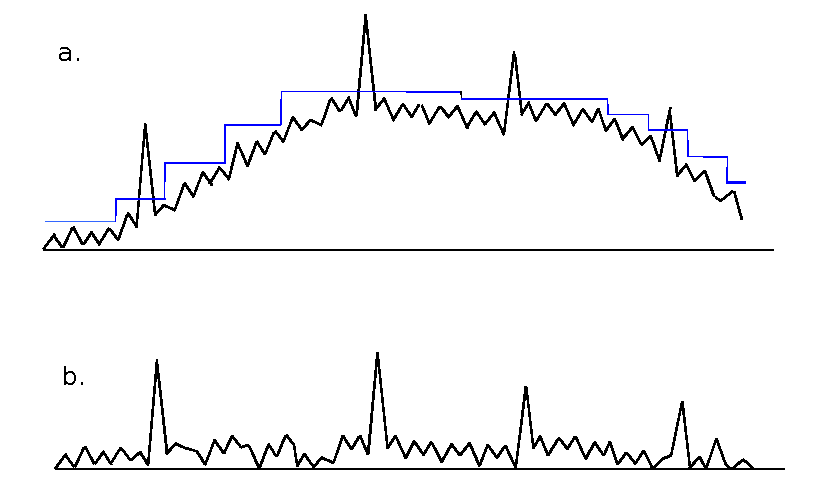
\includegraphics[width=4.16667in,height=\textheight]{figs/cfar-signal.pdf}
\caption{The signal level within one pulse window: a) before CFAR; b)
after CFAR}\label{fig:cfar-signal}
}
\end{figure}

\begin{Shaded}
\begin{Highlighting}[numbers=left,,firstnumber=411,]
\OtherTok{fCFAR ::} \DataTypeTok{Range}\NormalTok{ (}\DataTypeTok{Window} \DataTypeTok{RealData}\NormalTok{) }\OtherTok{->} \DataTypeTok{Range}\NormalTok{ (}\DataTypeTok{Window} \DataTypeTok{RealData}\NormalTok{)}
\NormalTok{fCFAR rbins }\FunctionTok{=}\NormalTok{ V.farm41 (\textbackslash{}m }\OtherTok{->}\NormalTok{ V.farm31 (normCfa m)) md rbins lmv emv}
  \KeywordTok{where}
\NormalTok{    md  }\FunctionTok{=}\NormalTok{ V.farm11 (}\FunctionTok{logBase} \DecValTok{2} \FunctionTok{.}\NormalTok{ V.reduce }\FunctionTok{min}\NormalTok{) rbins}
\NormalTok{    emv }\FunctionTok{=}\NormalTok{ (V.fanoutn (nFFT }\FunctionTok{+} \DecValTok{1}\NormalTok{) dummy) }\FunctionTok{<++>}\NormalTok{ (V.farm11 aritMean neighbors)}
\NormalTok{    lmv }\FunctionTok{=}\NormalTok{ (V.drop }\DecValTok{2} \FunctionTok{$}\NormalTok{ V.farm11 aritMean neighbors) }\FunctionTok{<++>}\NormalTok{ (V.fanout dummy) }
    \CommentTok{-----------------------------------------------}
\NormalTok{    normCfa m a l e }\FunctionTok{=} \DecValTok{2} \FunctionTok{**}\NormalTok{ (}\DecValTok{5} \FunctionTok{+} \FunctionTok{logBase} \DecValTok{2}\NormalTok{ a }\FunctionTok{-} \FunctionTok{maximum}\NormalTok{ [l,e,m])}
\OtherTok{    aritMean ::} \DataTypeTok{Vector}\NormalTok{ (}\DataTypeTok{Vector} \DataTypeTok{RealData}\NormalTok{) }\OtherTok{->} \DataTypeTok{Vector} \DataTypeTok{RealData}
\NormalTok{    aritMean  }\FunctionTok{=}\NormalTok{ V.farm11 (}\FunctionTok{/}\NormalTok{n) }\FunctionTok{.}\NormalTok{ V.reduce addV }\FunctionTok{.}\NormalTok{ V.farm11 geomMean }\FunctionTok{.}\NormalTok{ V.group }\DecValTok{4}
\NormalTok{    geomMean  }\FunctionTok{=}\NormalTok{ V.farm11 (}\FunctionTok{logBase} \DecValTok{2} \FunctionTok{.}\NormalTok{ (}\FunctionTok{/}\DecValTok{4}\NormalTok{)) }\FunctionTok{.}\NormalTok{ V.reduce addV}
    \CommentTok{-----------------------------------------------}
\NormalTok{    dummy     }\FunctionTok{=}\NormalTok{ V.fanoutn nFFT }\FunctionTok{$}\NormalTok{ (}\FunctionTok{-}\NormalTok{maxFloat)}\FunctionTok{/}\NormalTok{n}
\NormalTok{    neighbors }\FunctionTok{=}\NormalTok{ V.stencil nFFT rbins}
    \CommentTok{-----------------------------------------------}
\NormalTok{    addV      }\FunctionTok{=}\NormalTok{ V.farm21 (}\FunctionTok{+}\NormalTok{)}
\NormalTok{    n         }\FunctionTok{=} \FunctionTok{fromIntegral}\NormalTok{ nFFT}
\end{Highlighting}
\end{Shaded}

\begin{longtable}[]{@{}lll@{}}
\toprule
Function & Original module & Package\tabularnewline
\midrule
\endhead
\texttt{farm}{[}\texttt{4}/\texttt{3}/\texttt{1}{]}\texttt{1},
\texttt{reduce}, \texttt{\textless{}++\textgreater{}}, &
\href{https://forsyde.github.io/forsyde-atom/api/ForSyDe-Atom-Skeleton-Vector.html}{\texttt{ForSyDe.Atom.Skeleton.Vector}}
& forsyde-atom\tabularnewline
\texttt{drop}, \texttt{fanout}, \texttt{fanoutn}, \texttt{stencil} &
&\tabularnewline
\texttt{comb11} &
\href{https://forsyde.github.io/forsyde-atom/api/ForSyDe-Atom-MoC-SDF.html}{\texttt{ForSyDe.Atom.MoC.SDF}}
& forsyde-atom\tabularnewline
\texttt{maxFloat} & ForSyDe.AESA.Coefs & aesa-atom\tabularnewline
\texttt{nb}, \texttt{nFFT} & \texttt{ForSyDe.AESA.Params} &
aesa-atom\tabularnewline
\bottomrule
\end{longtable}

The \(f_{CFAR}\) function itself can be described with the system of
eq.~\ref{eq:cfar}, where

\begin{itemize}
\item
  \(MD\) is the minimum value over all Doppler channels in a batch for a
  specific data channel and range bin.
\item
  \(EMV\) and \(LMV\) calculate the early and respectively late mean
  values from the neighboring range bins as a combination of geometric
  and arithmetic mean values.
\item
  \(eb\) and \(lb\) are the earliest bin, respectively latest bin for
  which the CFAR can be calculated as \(EMV\) and \(LMV\) require at
  least \(N_{FFT}\) bins + 1 guard bin before and respectively after the
  current bin. This phenomenon is also called the ``stencil halo'',
  which means that CFAR, as defined in eq.~\ref{eq:cfar} is applied only
  on \(N_b'=N_b-2N_{FFT}-2\) bins.
\item
  bins earlier than \(eb\), respectively later than \(lb\), are ingnored
  by the CFAR formula and therefore their respective EMV and LMV are
  replaced with the lowest representable value.
\item
  5 is added to the exponent of the CFAR equation to set the gain to 32
  (i.e.~with only noi se in the incoming video the output values will be
  32).
\end{itemize}

\begin{equation}\begin{aligned}&\left\{\begin{aligned}
  &CFAR(a_{ij})= 2^{(5 + \log_2 a_{ij}) - \max (EMV(a_{ij}),LMV(a_{ij}),MD(a_{ij}))}\\
  &EMV(a_{ij}) = \frac{1}{N}\sum_{k=0}^{N-1}\left(\log_2\left(\frac{1}{4}\sum_{l=0}^{3}a_{(i-2-4k-l)j}\right)\right)\\
  &LMV(a_{ij}) = \frac{1}{N}\sum_{k=0}^{N-1}\left(\log_2\left(\frac{1}{4}\sum_{l=0}^{3}a_{(i+2+4k+l)j}\right)\right)\\
  &MD(a_{ij})  = \log_{2}\left(\min_{k=1}^N(a_{ik})\right)
  \end{aligned}\right.\\
  &\qquad \forall i\in[eb,lb], j\in[1,N] \text{ where }\left\{
  \begin{aligned}
  &N = N_{FFT}\\
  &eb = N_{FFT} + 1\\
  &lb = N_b - N_{FFT} - 1\\
  \end{aligned}\right.
  \end{aligned}
\label{eq:cfar}\end{equation}

The first thing we calculate is the \(MD\) for each Doppler window
(row). For each row of \texttt{rbins} (i.e.~range bins of Doppler
windows) we look for the minimum value (\texttt{reduceV\ min}) and apply
the binary logarithm on it.

Another action performed over the matrix \texttt{rbins} is to form two
stencil ``cubes'' for EMV and LMV respectively, by gathering batches of
\(N_{FFT}\) Doppler windows like in eq.~\ref{eq:cfar-stencil}, computing
them like in eq.~\ref{eq:cfar-emv}.

\begin{equation}
  \stackrel{\mbox{rbins}}{
  \begin{bmatrix}
  a_{11} & a_{12} & \cdots & a_{1N_{FFT}} \\
  a_{21} & a_{22} & \cdots & a_{2N_{FFT}} \\
  \vdots & \vdots & \ddots & \vdots \\
  a_{N_b1} & a_{N_b2} & \cdots & a_{N_bN_{FFT}}
  \end{bmatrix}}
  \stackrel{\mathtt{stencil}}{\rightarrow}
  \stackrel{\mbox{neighbors}}{
  \begin{bmatrix}
  \begin{bmatrix}
  a_{11} & a_{12} & \cdots & a_{1N_{FFT}} \\
  \vdots & \vdots & \ddots & \vdots \\
  a_{N_{FFT}1} & a_{N_{FFT}2} & \cdots & a_{N_{FFT}N_{FFT}} \\
  \end{bmatrix}\\
  \begin{bmatrix}
  a_{21} & a_{22} & \cdots & a_{2N_{FFT}} \\
  \vdots & \vdots & \ddots & \vdots \\
  a_{(N_{FFT}+1)1} & a_{(N_{FFT}+1)2} & \cdots & a_{(N_{FFT}+1)N_{FFT}} \\
  \end{bmatrix}\\
  \vdots \\
  \begin{bmatrix}
  a_{(N_b-N_{FFT})1} & a_{(N_b-N_{FFT})2} & \cdots & a_{(N_b-N_{FFT})N_{FFT}}\\
  \vdots & \vdots & \ddots & \vdots \\
  a_{N_b1} & a_{N_b2} & \cdots & a_{N_bN_{FFT}}
  \end{bmatrix}
  \end{bmatrix}}
\label{eq:cfar-stencil}\end{equation}

Each one of these neighbors matrices will constitute the input data for
calculating the \(EMV\) and \(LMV\) for each Doppler window. \(EMV\) and
\(LMV\) are calculated by applying the mean function \texttt{arithMean}
over them, as shown (only for the window associated with the \(eb\) bin)
in eq.~\ref{eq:cfar-emv}. The resulting \texttt{emv} and \texttt{lmv}
matrices are padded with rows of the minimum representable value
\texttt{-maxFloat}, so that they align properly with \texttt{rbins} in
order to combine into the 2D farm/stencil defined at eq.~\ref{eq:cfar}.
Finally, \texttt{fCFAR} yields a matrix of normalized Doppler windows.
The resulting matrices are not transformed back into sample streams by
the parent process, but rather they are passed as single tokens
downstream to the INT stage, where they will be processed as such.

\begin{equation}\begin{aligned}
  &\begin{bmatrix}
  a_{11} & \cdots & a_{1N_{FFT}} \\
  \vdots  & \ddots & \vdots \\
  a_{N_{FFT}1}  & \cdots & a_{N_{FFT}N_{FFT}}
  \end{bmatrix}
  \stackrel{\mathtt{group}}{\rightarrow}
  \begin{bmatrix}
  \begin{bmatrix}
  a_{11} & \cdots & a_{1N_{FFT}} \\
  \vdots & \ddots & \vdots \\
  a_{41} & \cdots & a_{4N_{FFT}}
  \end{bmatrix}\\
  \vdots \\
  \begin{bmatrix}
  a_{(N_{FFT}-4)1}  & \cdots & a_{(N_{FFT}-4)N_{FFT}}\\
  \vdots & \ddots & \vdots \\
  a_{N_{FFT}1}  & \cdots & a_{N_{FFT}N_{FFT}}
  \end{bmatrix}
  \end{bmatrix}\\
  &\stackrel{\mathtt{farm(geomMean)}}{\rightarrow}
  \begin{bmatrix}
  \log_2\frac{1}{4}\sum_{i=1}^{4}a_{i1} & \cdots & \log_2\frac{1}{4}\sum_{i=1}^{4}a_{iN_{FFT}} \\
  \vdots & \ddots & \vdots \\
  \log_2\frac{1}{4}\sum_{i=N_{FFT}-4}^{N_{FFT}}a_{i1} & \cdots & \log_2\frac{1}{4}\sum_{i=N_{FFT}-4}^{N_{FFT}}a_{iN_{FFT}}
  \end{bmatrix}\\
  &\stackrel{\mathtt{(/N_{FFT})\circ reduce(+)}}{\rightarrow}
  \begin{bmatrix}
  EMV(a_{eb,1}) & \cdots & EMV(a_{eb,N_{FFT}}) 
  \end{bmatrix}
  \end{aligned}
\label{eq:cfar-emv}\end{equation}

\hypertarget{sec:int-atom}{%
\paragraph{Integrator (INT)}\label{sec:int-atom}}

During the last stage of the video processing chain each data sample of
the video cube is integrated against its 8 previous values using an
8-tap FIR filter, as suggested by the drawing in
Figure~\ref{fig:int-cube-atom}.

\begin{figure}
\hypertarget{fig:int-cube-atom}{%
\centering
\includegraphics{figs/int-cube.pdf}
\caption{Integration on cubes of complex
samples}\label{fig:int-cube-atom}
}
\end{figure}

The integration depicted in Figure~\ref{fig:int-cube-atom}, like each
stage until now, can be modeled in dozens of different ways based on how
the designer envisions the partitioning of the data ``in time'' or ``in
space''. This partitioning could be as coarse-grained as streams of
cubes of samples, or as fine-grained as networks of streams of indvidual
samples. For convenience and for simulation efficiency\footnote{we try
  to avoid unnecessary transposes (i.e.~type traversals) which are
  time-consuming.} we choose a middle approach: video cubes are
represented as farms (i.e.~vectors) of streams of matrices, as
conveniently bundled by the previous DFB stages. We pass the
responsibility of re-partitioning and interpreting the data accordingly
to the downstream process, e.g.~a control/monitoring system, or a
testbench sink.

\begin{Shaded}
\begin{Highlighting}[numbers=left,,firstnumber=572,]
\OtherTok{int ::} \DataTypeTok{Beam}\NormalTok{ (}\DataTypeTok{SDF.Signal}\NormalTok{ (}\DataTypeTok{Range}\NormalTok{ (}\DataTypeTok{Window} \DataTypeTok{RealData}\NormalTok{)))}
    \OtherTok{->} \DataTypeTok{Beam}\NormalTok{ (}\DataTypeTok{SDF.Signal}\NormalTok{ (}\DataTypeTok{Range}\NormalTok{ (}\DataTypeTok{Window} \DataTypeTok{RealData}\NormalTok{)))}
    \OtherTok{->} \DataTypeTok{Beam}\NormalTok{ (}\DataTypeTok{SY.Signal}\NormalTok{  (}\DataTypeTok{Range}\NormalTok{ (}\DataTypeTok{Window} \DataTypeTok{RealData}\NormalTok{)))}
\NormalTok{int }\FunctionTok{=}\NormalTok{ V.farm21 procINT}
\end{Highlighting}
\end{Shaded}

Before integrating though, the data from both the left and the right
channel need to be merged. This is done by the process \texttt{merge}
below, which consumes one (matrix) token from each channel and
interleaves them at its output. When considering only abstract tokens,
the \texttt{merge} process can be regarded as an up-sampler with the
rate 2/1. When taking into consideration the size of the entire data set
(i.e.~token rates \(\times\) structure sizes \(\times\) data size), we
can easily see that the overall required system bandwidth (ratio)
remains the same between the PC and INT stages,
i.e.~\(\frac{2\times N_B \times N_{b} \times N_{FFT}\times \mathit{size}(\mathtt{RealData})}{N_B \times N_{b} \times N_{FFT}\times \mathit{size}(\mathtt{CpxData})}=1/1\).
For the integration stage \texttt{firNet} it is more appropriate to
translate back to SY MoC semantics, hence the \texttt{toSY} domain
interface.

\begin{figure}
\hypertarget{fig:int-net-atom}{%
\centering
\includegraphics{figs/int-net.pdf}
\caption{INT network}\label{fig:int-net-atom}
}
\end{figure}

\begin{Shaded}
\begin{Highlighting}[numbers=left,,firstnumber=591,]
\OtherTok{procINT ::} \DataTypeTok{Fractional}\NormalTok{ a }\OtherTok{=>} \DataTypeTok{SDF.Signal}\NormalTok{ (}\DataTypeTok{Matrix}\NormalTok{ a) }\OtherTok{->} \DataTypeTok{SDF.Signal}\NormalTok{ (}\DataTypeTok{Matrix}\NormalTok{ a) }\OtherTok{->} \DataTypeTok{SY.Signal}\NormalTok{ (}\DataTypeTok{Matrix}\NormalTok{ a)}
\NormalTok{procINT cr }\FunctionTok{=}\NormalTok{ firNet mkIntCoefs }\FunctionTok{.}\NormalTok{ SDF.toSY }\FunctionTok{.}\NormalTok{ merge cr}
  \KeywordTok{where}
\NormalTok{    merge   }\FunctionTok{=}\NormalTok{ SDF.comb21 ((}\DecValTok{1}\NormalTok{,}\DecValTok{1}\NormalTok{), }\DecValTok{2}\NormalTok{, \textbackslash{}[r] [l] }\OtherTok{->}\NormalTok{ [r, l])}
\end{Highlighting}
\end{Shaded}

The 8-tap FIR filter used for integration is also a moving average, but
as compared to the \texttt{mav} function used in
section~\ref{sec:pc-atom}, the window slides in time domain, i.e.~over
streaming samples rather than over vector elements. To instantiate a FIR
system we use the \texttt{firSk} skeleton provided by the ForSyDe-Atom
utility libraries, which constructs the the well-recognizable FIR
pattern in Figure~\ref{fig:int-net-atom}, i.e.~a recur-farm-reduce
composition. In order to do so, \texttt{firSk} needs to know \emph{what}
to fill this template with, thus we need to provide as arguments its
``basic'' operations, which in our case are processes operating on
signals of matrices. In fact, \texttt{mav} itself is a
\emph{specialization} of the \texttt{firSk} skeleton, which defines its
basic operations as corresponding functions on vectors. This feature
derives from a powerful algebra of skeletons which grants them both
modularity, and the possibility to transform them into
semantically-equivalent forms, as we shall soon explore in
section~\ref{sec:refinement}.

\begin{Shaded}
\begin{Highlighting}[numbers=left,,firstnumber=609,]
\OtherTok{firNet ::} \DataTypeTok{Num}\NormalTok{ a }\OtherTok{=>} \DataTypeTok{Vector}\NormalTok{ a }\OtherTok{->} \DataTypeTok{SY.Signal}\NormalTok{ (}\DataTypeTok{Matrix}\NormalTok{ a) }\OtherTok{->} \DataTypeTok{SY.Signal}\NormalTok{ (}\DataTypeTok{Matrix}\NormalTok{ a)}
\NormalTok{firNet coefs }\FunctionTok{=}\NormalTok{ fir' addSM mulSM dlySM coefs}
  \KeywordTok{where}
\NormalTok{    addSM   }\FunctionTok{=}\NormalTok{ SY.comb21 (M.farm21 (}\FunctionTok{+}\NormalTok{))}
\NormalTok{    mulSM c }\FunctionTok{=}\NormalTok{ SY.comb11 (M.farm11 (}\FunctionTok{*}\NormalTok{c))}
\NormalTok{    dlySM   }\FunctionTok{=}\NormalTok{ SY.delay  (M.fanout }\DecValTok{0}\NormalTok{)}
\end{Highlighting}
\end{Shaded}

\begin{longtable}[]{@{}lll@{}}
\toprule
\begin{minipage}[b]{0.21\columnwidth}\raggedright
Function\strut
\end{minipage} & \begin{minipage}[b]{0.42\columnwidth}\raggedright
Original module\strut
\end{minipage} & \begin{minipage}[b]{0.28\columnwidth}\raggedright
Package\strut
\end{minipage}\tabularnewline
\midrule
\endhead
\begin{minipage}[t]{0.21\columnwidth}\raggedright
\texttt{farm21}\strut
\end{minipage} & \begin{minipage}[t]{0.42\columnwidth}\raggedright
\href{https://forsyde.github.io/forsyde-atom/api/ForSyDe-Atom-Skeleton-Vector.html}{\texttt{ForSyDe.Atom.Skeleton.Vector}}\strut
\end{minipage} & \begin{minipage}[t]{0.28\columnwidth}\raggedright
forsyde-atom\strut
\end{minipage}\tabularnewline
\begin{minipage}[t]{0.21\columnwidth}\raggedright
\texttt{farm21},\texttt{farm11},\texttt{fanout}\strut
\end{minipage} & \begin{minipage}[t]{0.42\columnwidth}\raggedright
ForSyDe.Atom.Skeleton.Vector.Matrix\strut
\end{minipage} & \begin{minipage}[t]{0.28\columnwidth}\raggedright
forsyde-atom-extensions\strut
\end{minipage}\tabularnewline
\begin{minipage}[t]{0.21\columnwidth}\raggedright
\texttt{firSk}\strut
\end{minipage} & \begin{minipage}[t]{0.42\columnwidth}\raggedright
ForSyDe.Atom.Skeleton.Vector.DSP\strut
\end{minipage} & \begin{minipage}[t]{0.28\columnwidth}\raggedright
forsyde-atom-extensions\strut
\end{minipage}\tabularnewline
\begin{minipage}[t]{0.21\columnwidth}\raggedright
\texttt{comb21},\texttt{comb11}\strut
\end{minipage} & \begin{minipage}[t]{0.42\columnwidth}\raggedright
\href{https://forsyde.github.io/forsyde-atom/api/ForSyDe-Atom-MoC-SDF.html}{\texttt{ForSyDe.Atom.MoC.SDF}}\strut
\end{minipage} & \begin{minipage}[t]{0.28\columnwidth}\raggedright
forsyde-atom\strut
\end{minipage}\tabularnewline
\begin{minipage}[t]{0.21\columnwidth}\raggedright
\texttt{mkFirCoefs}\strut
\end{minipage} & \begin{minipage}[t]{0.42\columnwidth}\raggedright
ForSyDe.AESA.Coefs\strut
\end{minipage} & \begin{minipage}[t]{0.28\columnwidth}\raggedright
aesa-atom\strut
\end{minipage}\tabularnewline
\bottomrule
\end{longtable}

\hypertarget{system-process-network-1}{%
\subsubsection{System Process Network}\label{system-process-network-1}}

Finally, when putting all the blocks together in an equation, we obtain
the system \texttt{aesa\textquotesingle{}} in
Figure~\ref{fig:aesa-net-atom}.

\begin{figure}
\hypertarget{fig:aesa-net-atom}{%
\centering
\includegraphics{figs/aesa-net-atom.pdf}
\caption{AESA network as black-box components}\label{fig:aesa-net-atom}
}
\end{figure}

\begin{Shaded}
\begin{Highlighting}[numbers=left,,firstnumber=633,]
\OtherTok{aesa' ::} \DataTypeTok{Antenna}\NormalTok{ (}\DataTypeTok{SY.Signal} \DataTypeTok{CpxData}\NormalTok{) }\OtherTok{->} \DataTypeTok{Beam}\NormalTok{ (}\DataTypeTok{SY.Signal}\NormalTok{ (}\DataTypeTok{Range}\NormalTok{ (}\DataTypeTok{Window} \DataTypeTok{RealData}\NormalTok{)))}
\NormalTok{aesa' video }\FunctionTok{=}\NormalTok{ int rCfar lCfar}
  \KeywordTok{where}
\NormalTok{    lCfar     }\FunctionTok{=}\NormalTok{ cfar }\FunctionTok{$}\NormalTok{ dfb lCt}
\NormalTok{    rCfar     }\FunctionTok{=}\NormalTok{ cfar }\FunctionTok{$}\NormalTok{ dfb rCt}
\NormalTok{    (rCt,lCt) }\FunctionTok{=}\NormalTok{ ct }\FunctionTok{$}\NormalTok{ pc }\FunctionTok{$}\NormalTok{ dbf video}
\end{Highlighting}
\end{Shaded}

Although completely functional and modular, the system depicted in
Figure~\ref{fig:aesa-net-atom} is not the most ``pleasant'' to look at.
For the sake of code elegance and to increase the potential of
simulation distribution (see section~\ref{sec:parallel-sim}), we refine
the system \texttt{aesa\textquotesingle{}} to avoid unnecessary
merging-splitting of vectors between stages. On the other hand, from the
point of view of sequential performance it does not really matter,
because these patterns are ``ignored'' (reduced) by Haskell's lazy
evaluation system which can easily identify them as compositions of
inverse functions. Once we understand that between PC and INT the
processing path is replicated for each beam generated by the DBF.
Therefore it is possible to fuse the related \texttt{farm} skeletons
into the much simpler and more elegant model from
Figure~\ref{fig:aesa-net-atom2}. As both models are
semantically-equivalent an automated or tool-assisted transformation
process should be trivial.

\begin{Shaded}
\begin{Highlighting}[numbers=left,,firstnumber=654,]
\OtherTok{aesa ::} \DataTypeTok{Antenna}\NormalTok{ (}\DataTypeTok{SY.Signal} \DataTypeTok{CpxData}\NormalTok{) }\OtherTok{->} \DataTypeTok{Beam}\NormalTok{ (}\DataTypeTok{SY.Signal}\NormalTok{ (}\DataTypeTok{Range}\NormalTok{ (}\DataTypeTok{Window} \DataTypeTok{RealData}\NormalTok{)))}
\NormalTok{aesa }\FunctionTok{=}\NormalTok{ V.farm11 pcToInt }\FunctionTok{.}\NormalTok{ dbf}
\end{Highlighting}
\end{Shaded}

\begin{Shaded}
\begin{Highlighting}[numbers=left,,firstnumber=657,]
\NormalTok{pcToInt beam }\FunctionTok{=} \KeywordTok{let}\NormalTok{ (rb,lb) }\FunctionTok{=}\NormalTok{ procCT }\FunctionTok{$}\NormalTok{ procPC }\FunctionTok{$}\NormalTok{ SY.toSDF beam}
\NormalTok{                   lCFAR   }\FunctionTok{=}\NormalTok{ procCFAR }\FunctionTok{$}\NormalTok{ procDFB lb}
\NormalTok{                   rCFAR   }\FunctionTok{=}\NormalTok{ procCFAR }\FunctionTok{$}\NormalTok{ procDFB rb}
               \KeywordTok{in}\NormalTok{  procINT rCFAR lCFAR}
\end{Highlighting}
\end{Shaded}

\begin{figure}
\hypertarget{fig:aesa-net-atom2}{%
\centering
\includegraphics{figs/aesa-net-atom2.pdf}
\caption{AESA network when fusing the related
\texttt{farm}s}\label{fig:aesa-net-atom2}
}
\end{figure}

\hypertarget{sec:consts-coefs-atom}{%
\subsection{Coefficients, constants and
parameters}\label{sec:consts-coefs-atom}}

This section briefly presents the constants and coefficients which have
been used until now, and which shall be further used throughout this
report.

\hypertarget{references}{%
\section*{References}\label{references}}
\addcontentsline{toc}{section}{References}

\hypertarget{refs}{}
\leavevmode\hypertarget{ref-backus-1978}{}%
Backus, John. 1978. ``Can Programming Be Liberated from the von Neumann
Style?: A Functional Style and Its Algebra of Programs.''
\emph{Communications of the ACM} 21 (8): 613--41.
\url{https://doi.org/10.1145/359576.359579}.

\leavevmode\hypertarget{ref-Benveniste03}{}%
Benveniste, Albert, Paul Caspi, Stephen A. Edwards, Nicolas Halbwachs,
Paul Le Guernic, and Robert de Simone. 2003. ``The Synchronous Languages
12 Years Later.'' \emph{Proceedings of the IEEE} 91 (1): 64--83.

\leavevmode\hypertarget{ref-Fischer-2003}{}%
Fischer, Jörg, Sergei Gorlatch, and Holger Bischof. 2003. ``Foundations
of Data-Parallel Skeletons.'' In \emph{Patterns and Skeletons for
Parallel and Distributed Computing}, edited by Fethi A. Rabhi and Sergei
Gorlatch, 1--27. Springer London.
\url{https://doi.org/10.1007/978-1-4471-0097-3_1}.

\leavevmode\hypertarget{ref-hutton-2016}{}%
Hutton, Graham. 2016. \emph{Programming in Haskell}. 2nd ed. New York,
NY, USA: Cambridge University Press.

\leavevmode\hypertarget{ref-lee-2015}{}%
Lee, Edward. 2015. ``The Past, Present and Future of Cyber-Physical
Systems: A Focus on Models.'' \emph{Sensors} 15 (3): 4837--69.
\url{https://doi.org/10.3390/s150304837}.

\leavevmode\hypertarget{ref-Lee18}{}%
Lee, Edward A. 2018. ``Models of Timed Systems.'' In \emph{Formal
Modeling and Analysis of Timed Systems}, edited by David N. Jansen and
Pavithra Prabhakar, 17--33. Cham: Springer International Publishing.

\leavevmode\hypertarget{ref-lee95}{}%
Lee, Edward A, and Thomas M Parks. 1995. ``Dataflow Process Networks.''
\emph{Proceedings of the IEEE} 83 (5): 773--801.

\leavevmode\hypertarget{ref-lee98}{}%
Lee, Edward A, and Alberto Sangiovanni-Vincentelli. 1998. ``A Framework
for Comparing Models of Computation.'' \emph{IEEE Transactions on
Computer-Aided Design of Integrated Circuits and Systems} 17 (12):
1217--29.

\leavevmode\hypertarget{ref-leeseshia-15}{}%
Lee, Edward A., and Sanjit A. Seshia. 2016. \emph{Introduction to
Embedded Systems: A Cyber-Physical Systems Approach}. Second Edition.
MIT Press. \url{http://leeseshia.org}.

\leavevmode\hypertarget{ref-Lipovaca11}{}%
Lipovača, Miran. 2011. \emph{Learn You a Haskell for Great Good!: A
Beginner's Guide}. 1st ed. San Francisco, CA, USA: No Starch Press.

\leavevmode\hypertarget{ref-sander-2004}{}%
Sander, I., and A. Jantsch. 2004. ``System Modeling and Transformational
Design Refinement in Forsyde.'' \emph{IEEE Transactions on
Computer-Aided Design of Integrated Circuits and Systems} 23 (1):
17--32. \url{https://doi.org/10.1109/tcad.2003.819898}.

\leavevmode\hypertarget{ref-Sifakis15}{}%
Sifakis, Joseph. 2015. ``System Design Automation: Challenges and
Limitations'' 103 (November): 2093--2103.

\leavevmode\hypertarget{ref-skillicorn05}{}%
Skillicorn, David B. 2005. \emph{Foundations of Parallel Programming}.
6. Cambridge University Press.

\leavevmode\hypertarget{ref-atom-manual}{}%
Ungureanu, George. 2018. \emph{ForSyDe-Atom User Manual}. KTH Royal
Institute of Technology.
\url{https://forsyde.github.io/forsyde-atom/assets/manual.pdf}.

\leavevmode\hypertarget{ref-ungureanu17}{}%
Ungureanu, George, and Ingo Sander. 2017. ``A Layered Formal Framework
for Modeling of Cyber-Physical Systems.'' In \emph{2017 Design,
Automation \& Test in Europe Conference \& Exhibition (Date)}, 1715--20.
IEEE.

\end{document}
